%% abtex2-modelo-trabalho-academico.tex, v-1.9 laurocesar
%% Copyright 2012-2013 by abnTeX2 group at http://abntex2.googlecode.com/ 
%% This work may be distributed and/or modified under the conditions of the LaTeX Project Public License, either version 1.3
%% of this license or (at your option) any later version. The latest version of this license is in www.latex-project.org/lppl.txt
%% and version 1.3 or later is part of all distributions of LaTeX version 2005/12/01 or later.
%% This work has the LPPL maintenance status `maintained'.
%% The Current Maintainer of this work is the abnTeX2 team, led by Lauro César Araujo. Further information are available on 
%% http://abntex2.googlecode.com/ 
%% This work consists of the files abntex2-modelo-trabalho-academico.tex, abntex2-modelo-include-comandos and abntex2-modelo-references.bib
% ------------------------------------------------------------------------

\documentclass[12pt,oneside,a4paper, chapter=TITLE, section = TITLE, english, brazil]{abntex2}

\usepackage{lmodern}			% Usa a fonte Latin Modern			
%\usepackage{txfonts}          % Usa a fonte Times New Roman
%\renewcommand{\rmdefault}{phv} % Arial
%\renewcommand{\sfdefault}{phv}
\usepackage[T1]{fontenc}		% Selecao de codigos de fonte.
\usepackage[utf8]{inputenc}		% Cod. do doc. (conversão auto. dos acentos)
\usepackage{lastpage}			% Usado pela Ficha catalográfica
\usepackage{indentfirst}		% Indenta o primeiro parágrafo de cada seção.
\usepackage{color}				% Controle das cores
\usepackage{graphicx}			% Inclusão de gráficos
\usepackage{microtype} 			% para melhorias de justificação
\usepackage[brazilian,hyperpageref]{backref}  % Pag. c/ as citações na bibl
\usepackage[alf]{abntex2cite}	% Citações padrão ABNT
%\usepackage{geometry}
%\geometry{lmargin=3.0cm,rmargin=2.0cm,tmargin=3.0cm,bmargin=2.0cm}
\usepackage{todonotes}

% --------------------- CONFIGURAÇÕES DE PACOTES --------------------------

% Configurações do pacote backref:
	% Usado sem a opção hyperpageref de backref
	\renewcommand{\backrefpagesname}{Citado na(s) página(s):~}
	% Texto padrão antes do número das páginas
	\renewcommand{\backref}{}
	% Define os textos da citação
	\renewcommand*{\backrefalt}[4]{
		\ifcase #1 %
			Nenhuma citação no texto.%
		\or
			Citado na página #2.%
		\else
			Citado nas páginas #2.%
		\fi}%


% ---------- INFORMAÇÕES DE DADOS PARA CAPA E FOLHA DE ROSTO ---------------
\titulo{CONTROLE DE UM SISTEMA DE MANIPULAÇÃO PARA UM ROBÔ DE INSPEÇÃO EM LINHAS DE ALTA TENSÃO}
\autor{BRUNO QUEIROZ GAMA}
\local{Salvador}
\data{Março, 2014}
\orientador{Prof. MSc. Marco Antonio dos Reis}  
%\coorientador{Adeílson Fábio Correia}
\instituicao{Faculdade de Tecnologia SENAI CIMATEC}
\tipotrabalho{Trabalho de Conclusão de Curso}
\preambulo{Trabalho de conclusão de curso apresentado ao Curso de Especialização em Automação e Controle
da Faculdade de Tecnologia SENAI-CIMATEC como parte dos requisitos para a 
obtenção do título de Especialista em Controle, Automação e Robótica.}

% ------------ CONFIGURAÇÕES DE APARÊNCIA DO PDF FINAL -------------------

\definecolor{blue}{RGB}{41,5,195} % alterando o aspecto da cor azul

% informações do PDF
\makeatletter
\hypersetup{
     	%pagebackref=true,
		pdftitle={\@title}, 
		pdfauthor={\@author},
    	pdfsubject={\imprimirpreambulo},
	    pdfcreator={LaTeX with abnTeX2},
		pdfkeywords={abnt}{latex}{abntex}{abntex2}{trabalho acadêmico}, 
		colorlinks=true,       		% false: boxed links; true: colored links
    	linkcolor=blue,          	% color of internal links
    	citecolor=blue,        		% color of links to bibliography
    	filecolor=magenta,      	% color of file links
		urlcolor=blue,
		bookmarksdepth=4
}

%Criação do símbolo de fase (notação de circuitos)
\def\phase#1{{\vbox{\ialign{$\m@th\scriptstyle##$\crcr
			 \not\mathrel{\mkern10mu\smash{#1}}\crcr
			 \noalign{\nointerlineskip}
			 \mkern2.5mu\leaders\hrule height.34pt\hfill\mkern2.5mu\crcr}}}}
			 
\makeatother

% --------------- ESPAÇAMENTOS ENTRE LINHAS E PARÁGRAFOS ----------------- 

\setlength{\parindent}{1.3cm}  % Tamanho do parágrafo
\setlength{\parskip}{0.2cm}  % Espaçamento entre parágrafos

% ------------------------ COMPILA O ÍNDICE ------------------------------
\makeindex

% ----------------------- INÍCIO DO DOCUMENTO ----------------------------

\begin{document}

% ------------------------------------------------------------------------
%                          ELEMENTOS PRÉ-TEXTUAIS
% ------------------------------------------------------------------------

% -------------------------------- CAPA ----------------------------------

\begin{capa}
\begin{center}
	
\includegraphics[scale=.5]{imagens/logo_senai} \\
	\begin{large}
		\textbf{FACULDADE DE TECNOLOGIA SENAI CIMATEC \\ 
		ESPECIALIZAÇÃO EM CONTROLE, AUTOMAÇÃO E ROBÓTICA}
 		\vfill % Ajuste vertical
 		\textbf{\imprimirautor}
 		\vfill %Ajuste vertical
 		\begin{Large}
 			\textbf{\imprimirtitulo}
 		\end{Large}
  		\vfill
	\end{large}
 
 \imprimirlocal \\
 \imprimirdata

\end{center}  

\newpage

\frenchspacing % Retira espaço extra obsoleto entre as frases.
\end{capa}

% ---------------------------- FOLHA DE ROSTO ----------------------------

\begin{folhaderosto}
\begin{center}
	\textbf{\imprimirautor}
	\vfill
	\textbf{\imprimirtitulo}
	\vfill
	\begin{flushright}		
		\begin{minipage}{10cm}
			\imprimirpreambulo			
			\\ 
			\\
			Orientador: \imprimirorientador \\
			%Coorientador: \imprimircoorientador
		\end{minipage}				
	\end{flushright}
	\vfill
	\imprimirlocal \\
	\imprimirdata
\end{center}
\newpage
\end{folhaderosto}

% ------------------------- FICHA BIBLIOGRÁFICA --------------------------

\begin{fichacatalografica}
% A biblioteca da sua universidade fornecerá um PDF com a ficha catalográfica definitiva após a defesa do trabalho. Quando estiver com o documento, salve-o como PDF no diretório do seu projeto e substitua todo o conteúdo de implementação deste arquivo pelo comando abaixo:

% \begin{fichacatalografica}
%     \includepdf{fig_ficha_catalografica.pdf}
% \end{fichacatalografica}

	\vspace*{\fill}					% Posição vertical
	\hrule							% Linha horizontal
	\begin{center}					% Minipage Centralizado
	\begin{minipage}[c]{12.5cm}		% Largura
	
	\imprimirautor
	
	\hspace{0.5cm} \imprimirtitulo  / \imprimirautor. --
	\imprimirlocal, \imprimirdata-
	
	\hspace{0.5cm} \pageref{LastPage} p. : il. (algumas color.) ; 30 cm.\\
	
	\hspace{0.5cm} \imprimirorientadorRotulo~\imprimirorientador\\
	
	\hspace{0.5cm}
	\parbox[t]{\textwidth}{\imprimirtipotrabalho~--~\imprimirinstituicao,
	\imprimirdata.}\\
	
	\hspace{0.5cm}
		1. Palavra-chave1.
		2. Palavra-chave2.
		I. Orientador.
		II. Universidade xxx.
		III. Faculdade de xxx.  
		IV. Título\\ 			
	
	\hspace{8.75cm} CDU 02:141:005.7\\
	
	\end{minipage}
	\end{center}
	\hrule
	\newpage
	\end{fichacatalografica}

% -------------------------- FOLHA DE APROVAÇÃO --------------------------

\begin{folhadeaprovacao}
% Você pode utilizar este modelo até a aprovação do trabalho. Após isso, substitua todo o conteúdo deste arquivo por uma imagem da página assinada pela banca com o comando abaixo:

% \includepdf{folhadeaprovacao_final.pdf}

\begin{center}
	\imprimirautor
	\vfill
	\imprimirtitulo
\end{center}
\vfill
\imprimirpreambulo \\
\begin{flushright}
	Aprovado em \today .
\end{flushright}
\ \\
\begin{center}
	\textbf{Banca Examinadora}	\\ \ \\
\end{center}
	Marco Antonio Reis - Orientador \hrulefill
	\\
	Mestre em Produtividade pela Universidade Federal de Santa Catarina, Florianópolis, Brasil \\
	\imprimirinstituicao \\ \ \\
	CONVIDADO I \hrulefill \\
	FORMAÇÃO (COMO PARA O ORIENTADOR) \\
	INSTITUICAO DO CONVIDADO I \\ \ \\
	CONVIDADO II \hrulefill \\
	FORMAÇÃO (COMO PARA O ORIENTADOR) \\
	INSTITUIÇÃO DO CONVIDADO II	
	\vfill
\begin{center}	
	\imprimirdata
\end{center}
\newpage
\end{folhadeaprovacao}

% ----------------------------- DEDICATÓRIA ------------------------------

\begin{dedicatoria}
\vfill 
\vspace*{\fill}
\noindent
\begin{flushright}
	Texto da dedicatória.
\end{flushright}
\newpage 
\end{dedicatoria}

% ---------------------------- AGRADECIMENTOS ----------------------------

\begin{agradecimentos}
\begin{flushleft}
	Texto do agradecimento.
\end{flushleft}
\newpage
\end{agradecimentos}

% -------------------------------- RESUMO --------------------------------

\begin{resumo}
\setlength{\absparsep}{18pt} % ajusta o espaçamento dos parágrafos do resumo

Texto do Resumo.
\\
\\
\textbf{Palavras-chaves}: palavra1. palavra2. palavra3.
\newpage
\end{resumo}

% ------------------------------- ABSTRACT -------------------------------

\begin{resumo}[Abstract]
\begin{otherlanguage*}{english}

Abstract's text.
\\
\\ 
\textbf{Key-words}: word1. word2. word3.
\end{otherlanguage*}
\end{resumo}

% ------------------------- LISTA DE ILUSTRAÇÕES -------------------------

\pdfbookmark[0]{\listfigurename}{lof}
\listoffigures*
\cleardoublepage

% --------------------------- LISTA DE TABELAS ---------------------------
%\pdfbookmark[0]{\listtablename}{lot}
%\listoftables*
%\cleardoublepage

% ---------------------- LISTA DE ABREVIATURAS E SIGLAS ------------------

\begin{siglas}

  \item [CLP] Controlador Lógico Programável
  
  \item [FT] Função de Transferência
  
  \item [FTMA] Função de Transferência de Malha Aberta
  
  \item [FTMF] Função de Transferência de Malha Fechada
  
  \item [m] Metro
  
  \item [MA] Malha Aberta
  
  \item [MF] Malha Fechada
  
  \item [N] Newton
  
  \item [PID] Proporcional Integral Derivativo
  
  item [rad] Radiano
  
  \item [ROS] Robot Operating System
  
  \item [s] Segundo
  
  \item [SISO] Single Input, Single Output
  
  \item [$\omega$$_{s}$] Frequência de Amostragem dos Sensores de Posição e Velocidade
      
  \end{siglas}

% -------------------------- LISTA DE SÍMBOLOS ---------------------------
%\begin{simbolos}
%  \item[$ \Gamma $] Letra grega Gama
%  \item[$ \Lambda $] Lambda
%  \item[$ \zeta $] Letra grega minúscula zeta
%  \item[$ \in $] Pertence
%\end{simbolos}

% ------------------------------- SUMÁRIO --------------------------------
\pdfbookmark[0]{\contentsname}{toc}
\tableofcontents*
\cleardoublepage


%%%%%%%%%%%%%%%%%%%%%%%%%%%%%%%%%%%%%%%%%%%%%%%%%%%%%%%%%%%%%%%%%%%%%%%%%%%
%%%%%%%%%%%%%%%%%%%%%%%%%%%%%%%%%%%%%%%%%%%%%%%%%%%%%%%%%%%%%%%%%%%%%%%%%%%
%%%%%%%%%%%%%%%%%%%%%%%%%%%%%%%%%%%%%%%%%%%%%%%%%%%%%%%%%%%%%%%%%%%%%%%%%%%
%%%%%%%%%%%%%%%%%%%%%%%%%%%%%%%%%%%%%%%%%%%%%%%%%%%%%%%%%%%%%%%%%%%%%%%%%%%
%%%%%%%%%%%%%%%%%%%%%%%%%%%%%%%%%%%%%%%%%%%%%%%%%%%%%%%%%%%%%%%%%%%%%%%%%%
% ------------------------------------------------------------------------%
%							ELEMENTOS TEXTUAIS                            %
% ------------------------------------------------------------------------%
%%%%%%%%%%%%%%%%%%%%%%%%%%%%%%%%%%%%%%%%%%%%%%%%%%%%%%%%%%%%%%%%%%%%%%%%%%%
%%%%%%%%%%%%%%%%%%%%%%%%%%%%%%%%%%%%%%%%%%%%%%%%%%%%%%%%%%%%%%%%%%%%%%%%%%%
%%%%%%%%%%%%%%%%%%%%%%%%%%%%%%%%%%%%%%%%%%%%%%%%%%%%%%%%%%%%%%%%%%%%%%%%%%%
%%%%%%%%%%%%%%%%%%%%%%%%%%%%%%%%%%%%%%%%%%%%%%%%%%%%%%%%%%%%%%%%%%%%%%%%%%%
%%%%%%%%%%%%%%%%%%%%%%%%%%%%%%%%%%%%%%%%%%%%%%%%%%%%%%%%%%%%%%%%%%%%%%%%%%%


\textual

\chapter{INTRODUÇÃO} %Falta terminar

Atualmente as empresas tem encarado o desafio de modernizar e inovar em suas estruturas de produção e gestão sob o dever de se tornarem competitivos perante o mercado. Desta forma, a capacidade de realizar inovação tecnológica é extremamente necessária para emergir em mercados de alta concorrência. Seguindo este contexto, observa-se a necessidade crescente de engenheiros com conhecimento de técnicas avançadas em automação de linhas de fabricação e robótica \cite{rosario}.

Em frente ao dever de realizar o crescimento sustentável da sociedade, a automação e a robótica realizou o desenvolvimento e aumentou a eficiência dos processos industriais, no entanto, o mercado passou a exigir maior diversificação e menor tempo de desenvolvimento dos produtos, tornando a exigir maiores evoluções da automação e robótica \cite{rosario}.

Diante dessas necessidades de diversificação exigida pelo mercado mundial, algumas empresas e centros de pesquisa encontram-se com a aspiração de desenvolver novos produtos com nível de inovação e diversificação não encontrado no mercado. Este é caso do atual do SENAI - CIMATEC, que em seu laboratório de microeletrônica desenvolve um robô inovador para inspeção em linhas de transmissão de energia elétrica com alta tensão.

Além da utilização do robô em um campo de atuação a qual exige alta repetitividade e precisão, este produto proporcionará a segurança, visto que o profissional que realiza a inspeção das linhas de transmissão com alta tensão está exposto a um alto grau de periculosidade.

%Visando confeccionar este protótipo, insere-se este trabalho de conclusão de curso. Uma vez que o robô apresenta as unidades de apoio, tração e manipulação, enxerga-se a necessidade de projetar um sistema de controle de posição para a unidade de manipulação do robô, pois esta necessita de alta precisão em seus movimentos dado que a intercorrência de uma falha poderia causar um acidente.

Visando confeccionar este protótipo, insere-se este trabalho de conclusão de curso. Uma vez que o robô apresenta as unidades de apoio, tração e busca, enxerga-se a necessidade de projetar um sistema de controle de posição para as unidades do robô, pois este necessita de alta precisão em seus movimentos dado que a intercorrência de uma falha poderia causar um acidente. Desta forma, denominou-se de sistema de manipulação a parte que contem os servomotores, engrenagens e sensores que interliga as unidades de apoio e tração.

\todo{Falta terminar}

\section{OBJETIVOS} %FEITO

Este trabalho tem como objetivo principal realizar o controle de posição de três juntas presentes no sistema de manipulação de um robô atualmente desenvolvido pela equipe de microeletrônica do SENAI - CIMATEC. Este robô deverá realizar a inspeção de linhas de transmissão de energia elétrica em alta tensão, logo o controlador deve garantir uma precisão de posicionamento mínima para realização da atividade.

Como produto final deste trabalho de conclusão de curso, espera-se obter a equação do modelo mecânico dos motores e do robô e os ganhos \textit{(proporcinal, integral e derivativo)} dos controladores usados no sistema de manipulação do robô. Estes controladores deverão ser robustos o suficiente para que os servomotores dessa unidade siga as posições e velocidades de referência configuradas previamente.

\section{JUSTIFICATIVA} %FEITO

Sabe-se que é extremamente importante o controle de posição e velocidade de unidades que realizam o movimento de robôs, visto que a depender da aplicação desejada, estes não podem estar sujeito a uma alta possibilidade de falhas. Sob esta análise, um sistema de controle que atenda a todas as especificações de desempenho para o movimento do sistema de manipulação do robô é imprescindível para o andamento do projeto.

Entre outros motivos que comprovam a necessidade de um sistema de controle, podem ser acentuados a indispensabilidade de projetar um sistema em malha fechada que siga uma referência configurada pelo controlador com precisão, reduzindo a sensibilidade à variações de parâmetros, permitindo garantir a estabilidade e atenuando o feito de pertubações.

A realização deste trabalho sustenta-se pela necessidade presente de um sistema de controle de posição para o sistema de manipulação do robô desenvolvido pela equipe de microeletrônica do SENAI - CIMATEC. Este trabalho visa projetar um sistema de controle que atenda as especificações de movimento do robô para realização da inspeção com segurança e precisão em suas ações.

\section{METODOLOGIA} %FEITO

A metodologia aplicada para realização deste trabalho de conclusão de curso pode ser representada pelos seguintes passos:

\begin{enumerate}

\item Estudo de técnicas de modelagem de sistemas dinâmicos.

\item Ensaio experimental do servomotor Dynamixel MX-106R \textit{(utilizado para movimentar o sistema de manipulação do robô)}.

\item Modelagem do servomotor Dynamixel MX-106R. 

\item Projeto do controlador interno ao MX-106R a partir do modelo levantado anteriormente.

\item Modelagem via SolidWorks do sistema de manipulação do robô.

\item Projeto dos controladores externos ao servomotor Dynamixel MX-106R.

\item Simulação do modelo controlado via Matlab \textit{(Simulink)}.

\end{enumerate}

% % % % % % % % % % % % % % % % % % % % % % % % % % % % % % % % % %

\chapter{ROBÓTICA}

A palavra "robô"\ foi usada pela primeira vez pelo dramaturgo Karel Capek em 1921. Nessa época a palavra representava a realização do trabalho manual para seres humanos de forma perfeita e incansável. Posteriormente, na Europa, robótica foi definida como "os meios através dos quais robôs são colocados juntos e efetuando trabalho" \cite{fuller}.

Durante o século XIX, muitos robôs e sistemas automáticos foram desenvolvidos buscando reduzir o esforço braçal humano em tarefas inseguras e desagradáveis. Desta forma pôde-se dedicar esforços para a produção de atividades intelectuais \cite{silveira}.

Normalmente os robôs apresentam 3 tipos de componentes: partes físicas, instruções internas e instruções adaptáveis para tarefas. Nas partes físicas estão presentes 4 ou 5 unidades \cite{fuller}:

\begin{enumerate}

\item Estrutura mecânica

\item Atuadores

\item Sistema de Controle 

\item Ferramentas e Sensores

\item Console de controle manual

\end{enumerate}

Todo as ações do robô devem ser direcionados pela unidade de controle, de forma que seus movimentos sejam realizados da maneira e no tempo correto. Para dispor de segurança em todas essas ações, os sistemas devem funcionar em malha fechada \textit{(feedback de informação durante a realização da ação desejada)}.

Projetar um sistema de controle eficiente para atuar no movimento do sistema de manipulação requer uma análise precisa das características da estrutura mecânica, dos atuadores e dos sensores. Logo, realizar a modelagem das unidades que serão controladas é extremamente necessário para encontrar a melhor estratégia de controle do robô, uma vez que o sistema de manipulação é um conjunto de articulações a qual o movimento de uma junta influencia na posição de outra. Além disso, o modelo matemático do robô pode variar a depender os componentes utilizados \cite{sciavicco}.

%Os sensores são os elementos sensíveis aos fenômenos físicos como a pressão ou a temperatura de um fluido, enquanto que os atuadores são os mecanismos capazes de interagir no processo, alterando o valor das variáveis manipuláveis. Os controladores, por sua vez, são os dispositivos que, através do processamento dos dados obtidos pelos sensores e em função da programação pré-estabelecida, geram comandos para os atuadores.
%\cite{silveira}

\section{INSPEÇÃO EM LINHAS DE TRANSMISSÃO DE ENERGIA ELÉTRICA DE ALTA TENSÃO}

%BEN2013
No Brasil, segundo o Balanço Energético Nacional 2013, 16,9\% do consumo final de energia é proveniente da Eletricidade. Este valor considerável mostra a importância dessa energia para o funcionamento da industria, dos grandes centros urbanos e da população em geral. Logo, este teriam muitos problemas caso a transmissão dessa energia for interrompida, causando desconforto, prejuízo e outras adversidades.

%Eletrobras
Para transmitir a energia elétrica das usinas até os grandes centros consumidores, a energia percorre longas distâncias através das redes de transmissão. As redes de transmissão são compostas por cabos, torres e isoladores e, devido a sua importância, precisam receber manutenção frequentemente.

O aumento da demanda energética e recentes blackouts tem colocado pressão sobre os proprietários de redes de transmissão em melhorar a manutenção em seus sistemas. Desde então o número de iniciativas em desenvolver robôs para realização da inspeção em linhas de transmissão tem aumentado drasticamente \cite{transmission}.

A manutenção em linhas de transmissão de energia elétrica é um trabalho com elevado grau de risco, dado que é necessário que um profissional esteja suspenso na linha a cerca de 100 metros de altura. Durante a manutenção também é fundamental que o fornecimento de energia seja interrompido, para isso uma outra linha de transmissão é sobrecarregada para compensar a linha em manutenção \cite{expliner}.

Como opção para evitar submeter uma pessoa a um trabalho de imenso risco, entre outros métodos, existe a inspeção visual realizada através do uso de helicópteros auxiliado por algorítimos de reconhecimento de padrões. No entanto, esses método de inspeção são geralmente caros ou ainda assim apresentam risco \apud{expliner}{ishino}.

De acordo com \citeonline{expliner} e \citeonline{transmission}, uma alternativa para reduzir os custo e perigos da inspeção em linhas de transmissão é a utilização de robôs. No entanto, quanto maior a mobilidade desejada para o robô maior será peso, quando precisa-se de robôs leves para inspeção em linhas de transmissão.

%Hidro-Québec research institute
Desde 1998, Hidro Québec research institute (\cite{transmission}) tem intensificado o desenvolvimento de robôs aplicados à manutenção em linhas de transmissão. Seus protótipos são capazes de, em cerca de 1 segundo, ultrapassar obstáculos como: espaçadores, amortecedores e grampos de suspensão. Kansai Electric Power Corp. (KEPCO, Japan) e Japan Systems Corp. (JPS) (\cite{expliner}) também desenvolveram um robô de inspeção em linhas de transmissão capaz de se mover sobre os cabos de alta tensão, ultrapassar espaçadores de maneira segura e rápida e ultrapassar suspensões sem tocar na estrutura da torre.

%Existe outras informações no capítulo 8 (Finalidade do Processo) sobre a inspeção necessária

\section{ROBÔ IRoS - INSPECTION ROBOT SYSTEM (CEMIG)}

%Além da utilização do robô em um campo de atuação a qual exige alta repetitividade e precisão, este produto proporcionará a segurança, visto que o profissional que realiza a inspeção das linhas de transmissão com alta tensão está exposto a um alto grau de periculosidade.

%Visando confeccionar este protótipo, insere-se este trabalho de conclusão de curso. Uma vez que o robô apresenta as unidades de apoio, tração e manipulação, enxerga-se a necessidade de projetar um sistema de controle de posição para a unidade de manipulação do robô, pois esta necessita de alta precisão em seus movimentos dado que a intercorrência de uma falha poderia causar um acidente.

%Falar que tem algumas semelhanças com o robô "artigo - Transmission Line Maintenance...2.2.1 pg.4"

Atualmente encontra-se em desenvolvimento no laboratório de microeletrônica do SENAI - CIMATEC um robô para inspeção em linhas de transmissão de energia elétrica com alta tensão. O desenvolvimento deste robô busca realizar inovações em relação aos modelos atualmente encontrados no mercado.

Nomeado de robô IRoS, este foi idealizado em uma parceria de desenvolvimento entre o SENAI-CIMATEC e a CEMIG \textit{(Companhia Energética de Minas Gerais)}. Buscando sempre o caráter inovador neste desenvolvimento, o IRoS busca superar seus concorrente no mercado internacional em termos de autonomia, atividades de inspeção e peso.

% Citar o documento detalhado preliminar
O dispositivo robótico deverá estar apto a inspecionar linhas de transmissão com tensão entre 124,2 a 151,8 kV com corrente trifásica de 500 A, de forma autônoma, necessitando de operadores apenas para a sua instalação e remoção no trecho inspecionado ou por eventuais paradas de emergência. Ele será fixado ao cabo da linha viva através de garras, como pode ser observado na figura \ref{fig:robo} \cite{cemig}:

\begin{figure}[h] % Poderia ser \begin{figure}[posicionamento], onde o posicionamento pode ser h - no local do texto onde foi  o comando, t - no topo da pagina atual ou b - no final da pagina de trabalho.
\centering
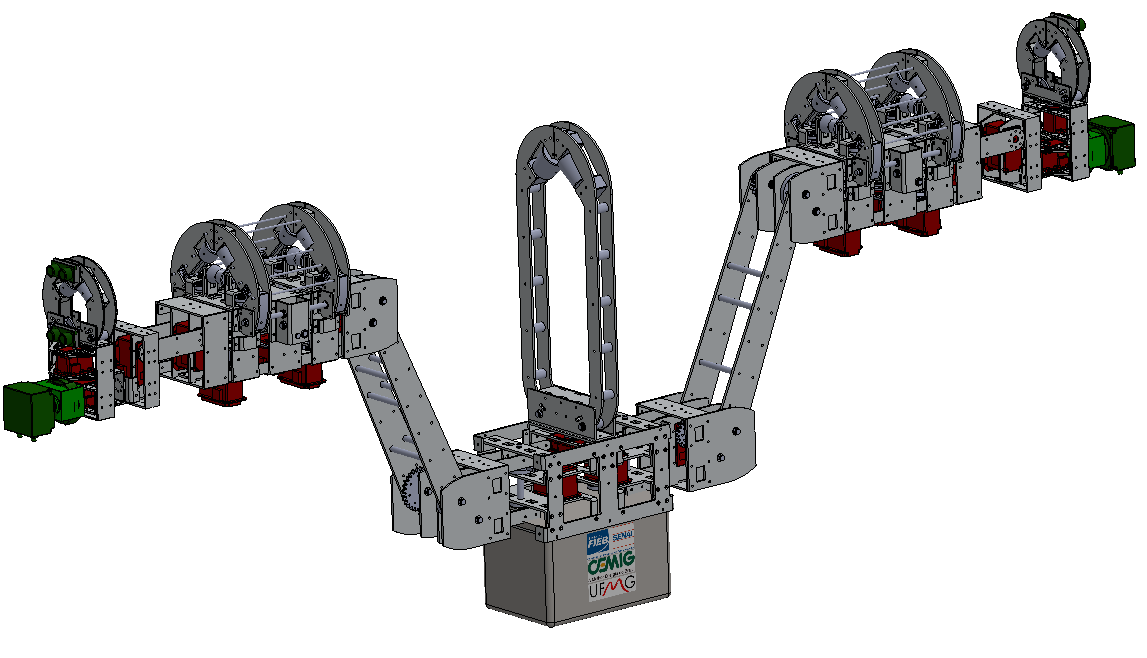
\includegraphics[scale=0.42]{./imagens/robo}
\caption[Estrutura mecãnica do sistema robótico proposto para inspeção de linhas vidas de 138 kV]{Estrutura mecãnica do sistema robótico proposto para inspeção de linhas vidas de 138 kV \cite{cemig}}
\label{fig:robo}
\end{figure}

O sistema robótico de inspeção pode ser dividido em 3 partes: Unidade de Busca, Unidade de Tração e Unidade de Apoio. Todas as unidades possuem garras para fixação do robô na linha. Uma melhor visualização das unidades pode ser visto na figura \ref{fig:unid_est_mec} \cite{cemig}.

\begin{figure}[h] % Poderia ser \begin{figure}[posicionamento], onde o posicionamento pode ser h - no local do texto onde foi  o comando, t - no topo da pagina atual ou b - no final da pagina de trabalho.
\centering
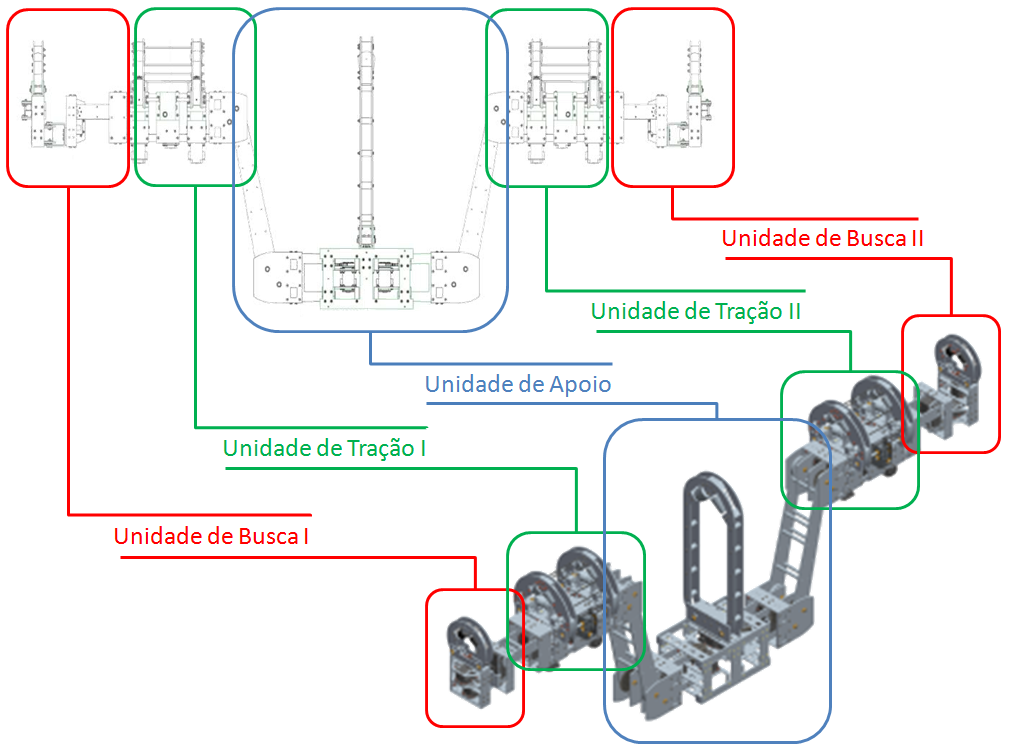
\includegraphics[scale=0.45]{./imagens/unidades_Robo}
\caption[Unidades da estrutura mecânica do sistema robótico porposto]{Unidades da estrutura mecânica do sistema robótico porposto \cite{cemig}}
\label{fig:unid_est_mec}
\end{figure}

A solução adotada para confecção do projeto propõe a divisão do robô em 8 sistemas \cite{cemig}:

\begin{enumerate}
\item Sistema de Acionamento;

\item Sistema de Comunicação Externa;

\item Sistema de Controle;

\item Sistema Mecânico;

\item Sistema de Potência;

\item Sistema de Processamento Central;

\item Sistema de Sensores;

\item Sistema de Visualização.

\end{enumerate}

Na figura \ref{fig:diagrama} pode ser visualizado o Diagrama da Arquitetura Geral do robô.

\ \\ \ \\

\begin{figure}[h] % Poderia ser \begin{figure}[posicionamento], onde o posicionamento pode ser h - no local do texto onde foi  o comando, t - no topo da pagina atual ou b - no final da pagina de trabalho.
\centering
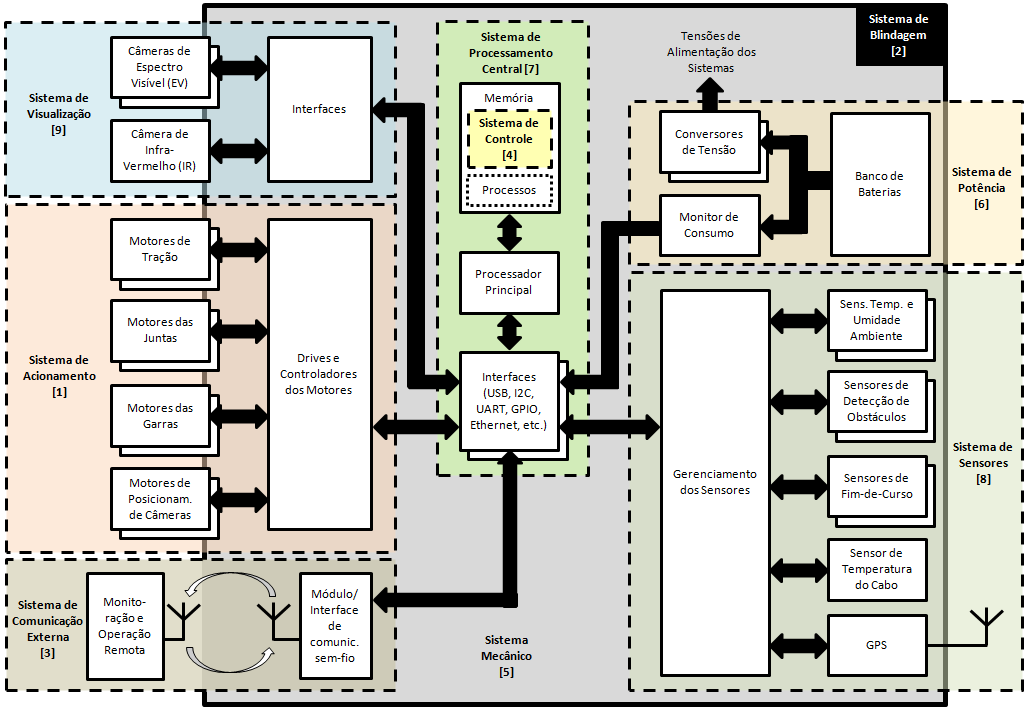
\includegraphics[scale=0.45]{./imagens/Diagrama_Completo}
\caption[Diagrama de Arquitetura Geral do robô de Inspeção de Linhas Vivas]{Diagrama de Arquitetura Geral do robô de Inspeção de Linhas Vivas \cite{cemig}}
\label{fig:diagrama}
\end{figure}

\subsection{SISTEMA DE CONTROLE DO ROBÔ IRoS}

O sistema de controle deve ser implementado a partir de algoritmos que elaborem estratégias de controle para que o robô se desloque na linha, ultrapasse obstáculos e realize as inspeções autonomamente a partir dos dados do Sistema de Sensores \cite{cemig}.

Segundo \apudonline{cemig}{siciliano}, a estratégia base para o controle do sistema robótico será a adoção de um controle de junta independente. Esta estratégia é descentralizada e as entradas de controle de cada junta apenas dependem do deslocamento e da velocidade da respectiva junta.

Através do controle de junta independente, é possível controlar cada eixo como um sistema SISO. Os efeitos gerados pelas engrenagens durante a realização dos movimentos, entre eles o \textbf{backlash}, são tratados como pertubações de saída \cite{cemig}.

\begin{citacao}
"Backlash é o motante pelo qual a largura do espaço do dente de uma engrenagem é superior à espessura de um dente de engate no diâmetro primitivo das engrenagens. Como a folga é proveniente da geometria circular das engrenagens, o backlash é uma quantidade angular" \apud{cemig}{backlash}.
\end{citacao}

O robô faz uso de engrenagens em seus eixos para atingir o torque necessário à realização do movimento pretendido. Observa-se então que essas engrenagens inserem folgas no sistema \textit{(backlash)}, de forma que posição indicada no encoder interno ao servomotor pode não representar a posição real das hastes. Portanto, observou-se a necessidade de implementar uma malha de controle fechado externo ao servomotor, uma vez que o controlador interno ao Dynamixel MX-106R não poderia garantir a posição desejada para as hastes do robô. A figura \ref{fig:malha_fechada} representa o sistema de controle implementado \cite{cemig}.

\begin{figure}[h] % Poderia ser \begin{figure}[posicionamento], onde o posicionamento pode ser h - no local do texto onde foi  o comando, t - no topo da pagina atual ou b - no final da pagina de trabalho.
\centering
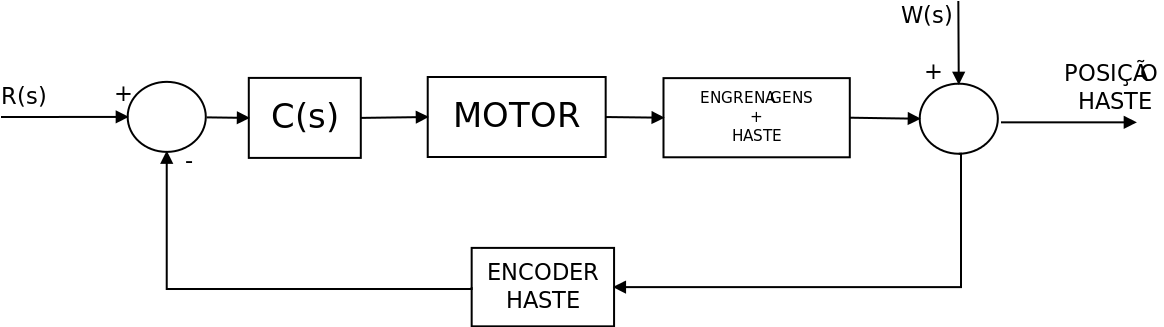
\includegraphics[scale=0.4]{./imagens/Malha_fechada}
\caption[Malha fechada para controle de posição de uma haste do robô]{Malha fechada para controle de posição de uma haste do robô \cite{cemig}}
\label{fig:malha_fechada}
\end{figure}

Sendo que R(s) representa a posição de referência, C(s) é a função de transferência do controlador projetado e W(s)  são as pertubações de saída.

% % % % % % % % % % % % % % % % % % % % % % % % % % % % % % % % % %

\chapter{MODELAGEM DE SISTEMAS DINÂMICOS}

Em função da necessidade de realizar o projeto do controlador do sistema de manipulação do robô IRoS, uma atividade preliminar muito importante é a modelagem matemática da dinâmica do sistema.

\begin{citacao}
"O modelo matemático de um sistema dinâmico é definido como um conjunto de equações que representa com precisão ou, pelo menos,  razoavelmente bem a dinâmica do sistema. Um sistema é representado de muitas maneiras diferentes e, portanto, pode ter vários modelos matemáticos, dependendo da perspectiva a ser considerada" \cite{ogata}.
\end{citacao}

É muito importante que o engenheiro de controle saiba regular uma conciliação entre a simplicidade do modelo e a precisão dos resultados da análise, pois a etapa mais importante na realização de sistemas de controle é a construção de modelos matemáticos \cite{ogata}.

O objetivo de encontrar o modelo dos sistemas dinâmicos é escolher os melhores parâmetros do controlador, de forma que a malha de controle execute bem o controle da variável do processo. A escolha dos melhores parâmetros do controlador podem ser escolhidos de duas formas diferentes. O primeiro método seria escolhendo alguns parâmetros, observando o comportamento do sistema e posteriormente ajustando-se os parâmetros até que o sistema apresente o comportamento desejado. O segundo método seria o desenvolvimento do modelo matemático que descreve o comportamento do sistema, e posteriormente, utilizar-se-ia técnicas de controle para escolher os parâmetros do controlador \cite{astrom}.

Por se tratar de um sistema eletro-mecânico, o robô IRoS necessita de modelagens matemáticas que identifique seus sistemas mecânicos e eletrônicos. Utiliza-se então a segunda lei de Newton \textit{(identificação mecânica)} e as leis das correntes e das tensões de Kirchhoff \textit{(identificação eletrônica)}.

O modelo dinâmico dos processos elétricos e mecânicos presentes no robô fornecerá a relação entre as entradas e saídas do sistema durante o regime transitório, período o qual é muito mais difícil extrair o comportamento do sistema. No entanto uma série de modelos podem ser aplicados para sistema lineares invariantes no tempo ou sistemas linearizados em um ponto de equilíbrio \cite{astrom}.

Segundo \citeonline{astrom}: "Em controle de processos, o degrau  é a resposta transiente mais usada para identificação de processos". Isto ocorre pois o degrau é o tipo de distúrbio mais fácil de ser gerado manualmente.

\section{MODELAGEM POR RESPOSTA AO DEGRAU} \label{sec:mod_degrau}

Segundo \citeonline{enso}, são recomendadas as seguintes etapas para realizar a identificação e modelagem de um sistema:

\begin{enumerate}

\item \textbf{Experimento ou Aquisição de dados:} Tem o objetivo de maximizar o volume das informações coletadas, dentro dos limites impostos pelo processo. Durante esta etapa o período de amostragem dos sensores devem ser suficientemente pequenos para que não ocorra perda de informação. Normalmente chama-se de $\omega_{s}$ a frequência de amostragem do sensor. Para evitar maiores problemas na aquisição de dados, a componente de frequência mais alta do processo deve ser menor que $\frac{\omega_{s}}{2}$;

\item \textbf{Seleção da estrutura do modelo:} Consiste em selecionar a ordem do modelo de forma que não seja simples o bastante para que não tenha dinâmicas não modeladas, mas também que não seja muito complexo dificultando realizar ações de controle;

\item \textbf{Estimação dos parâmetros:} Deve-se procurar estimar os parâmetros desconhecidos do modelo selecionado. A escolha dos parâmetros depende da estrutura do modelo selecionado bem como das propriedades das informações coletadas;

\item \textbf{Validação do modelo:} O método de validação depende das propriedades desejadas do modelo. Normalmente precisão e extrapolação são desejadas. A simulação será uma ferramenta muito útil para validação do modelo, análise de estabilidade e efeitos de pólos e zeros.

\end{enumerate}

A dinâmica de um sistema linear é representada pela sua resposta transitória, no entanto, necessita-se que o sistema esteja inicialmente em repouso. Modelos obtidos a partir de experimentos transitórios normalmente podem ser sintonizados por controladores PID \cite{astrom}.

Conforme \citeonline{astrom}, o ensaio experimental para aquisição de dados deve ser realizado da seguinte forma:

\begin{enumerate}

\item Espere que o processo esteja em repouso;

\item Configure o controlador para o modo manual \textit{(ensaio em malha aberta)};

\item Mude a variável de controle rapidamente;

\item Registre todas as variações do processo e normalize-as dividindo pelas variações da variável de controle;

\item Repita o ensaio para outros valores de amplitude do sinal de entrada e em diferentes condições de operação.

\end{enumerate}


Muitas características podem ser extraídas do sistema a partir do ensaio em malha aberta com entrada igual ao degrau. Informações como: estabilidade ou instabilidade em malha aberta, oscilação ao redor do valor estacionário, processos integradores, tempo morto, sistemas de fase não-mínima, entre outros, pode ser observado na figura \ref{fig:open_loop_resp}.

\begin{figure}[h] % Poderia ser \begin{figure}[posicionamento], onde o posicionamento pode ser h - no local do texto onde foi  o comando, t - no topo da pagina atual ou b - no final da pagina de trabalho.
\centering
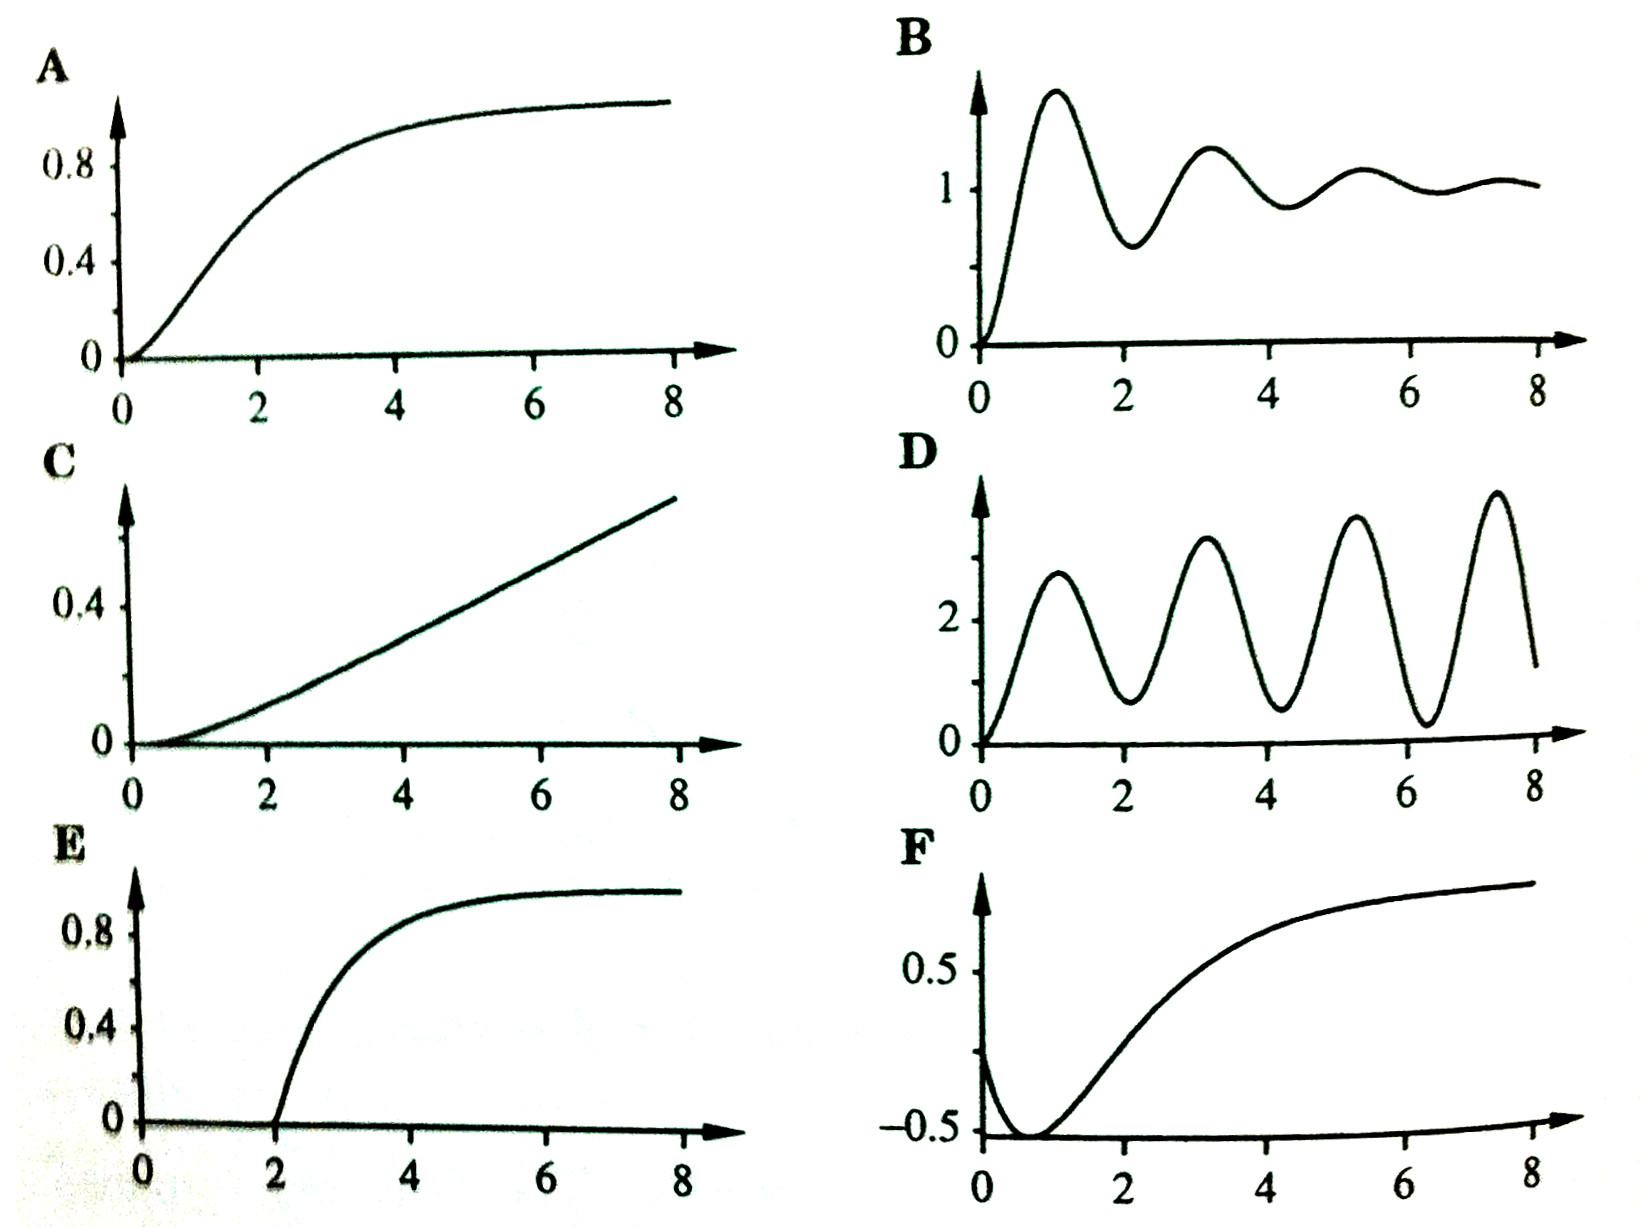
\includegraphics[scale=0.25]{./imagens/open_loop_resp}
\caption[Respostas em Malha Aberta]{Respostas em Malha Aberta \cite{astrom}}
\label{fig:open_loop_resp}
\end{figure}

Muitos métodos de sintonia e projeto de sistemas de controle são baseado na curva experimental de resposta ao degrau em malha aberta. Isto ocorre devido a sua simples interpretação física \cite{astrom}.

Muitos métodos de obtenção do modelo dinâmico de sistemas tem sido apresentado na literatura durante anos. Entre eles estão: modelo com dois, três e quatro parâmetros. Esses parâmetros podem ser extraídos a partir da resposta do sistema em malha aberta. Para sistemas lineares estes parâmetros serão constantes, porém para processos não-lineares, os parâmetros dependem das condições de operação \cite{astrom}.


\subsection{MODELO A DOIS PARÂMETROS} \label{sec:mod_2_param}

O modelo a dois parâmetros é a mais simples representação de um sistema. Sendo que o primeiro parâmetro é o ganho \textit{(K)} e o outro é a constante de tempo do sistema \textit{($\tau$)}. A depender da complexidade, este modelo pode representar de forma satisfatória o processo. O modelo a dois parâmetros pode ser representado pela equação \cite{astrom}:

\begin{equation}
G(s) = \frac{K}{1 + \tau s} \label{eq:g_de_s_2param}
\end{equation}

A resposta do processo, representado pela equação \ref{eq:g_de_s_2param}, à entrada degrau  pode ser observado na figura \ref{fig:resp_g_de_s_2param}.

\begin{figure}[h] % Poderia ser \begin{figure}[posicionamento], onde o posicionamento pode ser h - no local do texto onde foi  o comando, t - no topo da pagina atual ou b - no final da pagina de trabalho.
\centering
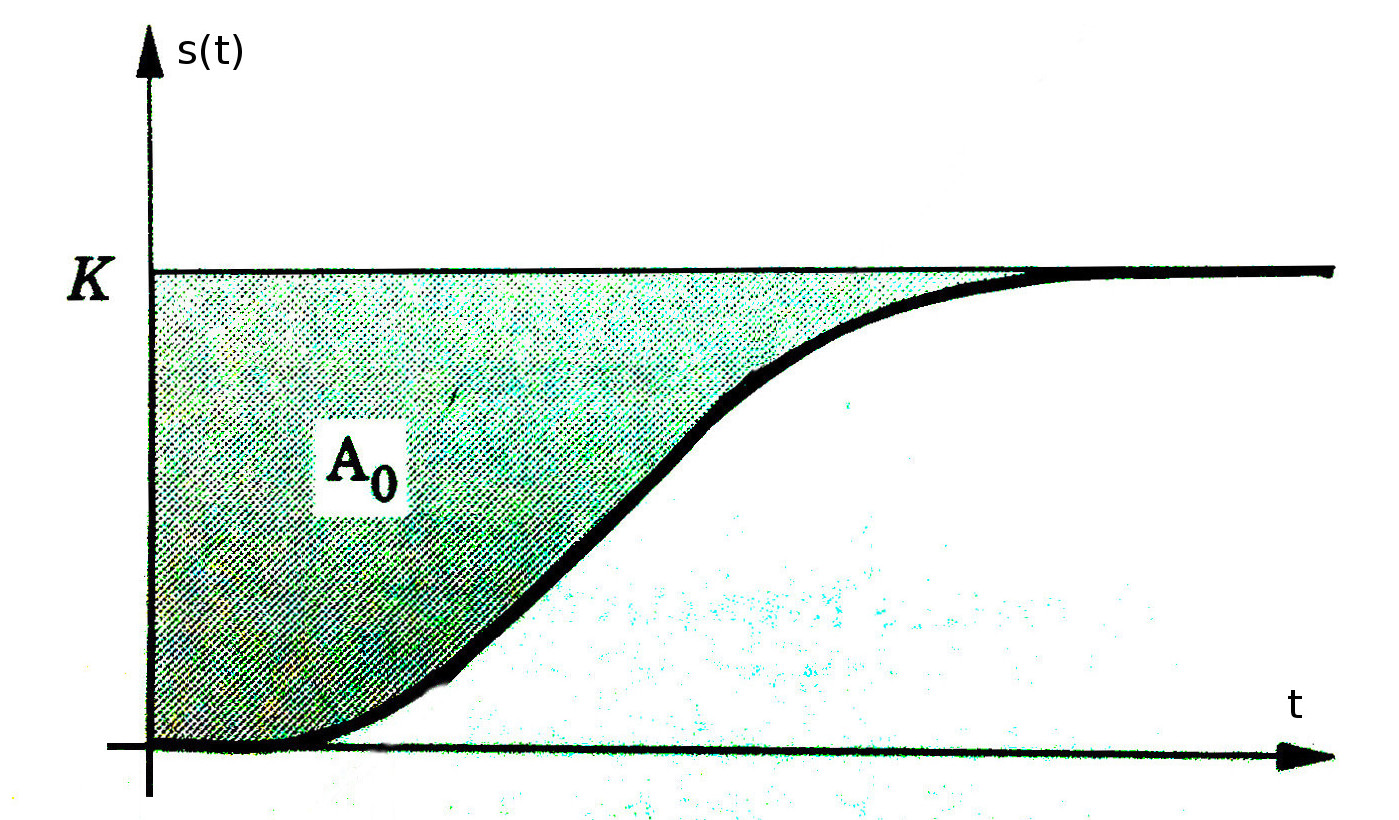
\includegraphics[scale=0.3]{./imagens/resp_g2}
\caption[Gráfico da resposta característica de um processo representado pela equação \ref{eq:g_de_s_2param}]{Gráfico da resposta característica de um processo representado pela equação \ref{eq:g_de_s_2param} \cite{astrom}}
\label{fig:resp_g_de_s_2param}
\end{figure}

Sendo que:
\begin{equation}
K = s(\infty) \label{eq:k_mod_2_param}
\end{equation}

\begin{equation}
A_{0} = \int^{+\infty}_0 (s(\infty) - s(t))dt \label{eq:tau_mod_2_param_1}
\end{equation}

\begin{equation}
\tau = \frac{A_{0}}{K} \label{eq:tau_mod_2_param_2}
\end{equation}

\subsection{MODELO A TRÊS PARÂMETROS}

De acordo com \citeonline{astrom}, a medida que se aumenta o número de parâmetros, melhores aproximações do sistema real podem ser obtidas. A equação \ref{eq:g_de_s_3param} representa o modelo a três parâmetros.

\begin{equation}
G(s) = \frac{K}{1 + \tau s}e^{-sL} \label{eq:g_de_s_3param}
\end{equation}

Sendo K o ganho estático do sistema, $\tau$ a constante de tempo e L o tempo morto. A resposta descrita pelo modelo da equação \ref{eq:g_de_s_3param} quando excitado pela entrada igual ao degrau pode ser observador pela figura \ref{fig:resp_g_de_s_3param}:

\begin{figure}[h] % Poderia ser \begin{figure}[posicionamento], onde o posicionamento pode ser h - no local do texto onde foi  o comando, t - no topo da pagina atual ou b - no final da pagina de trabalho.
\centering
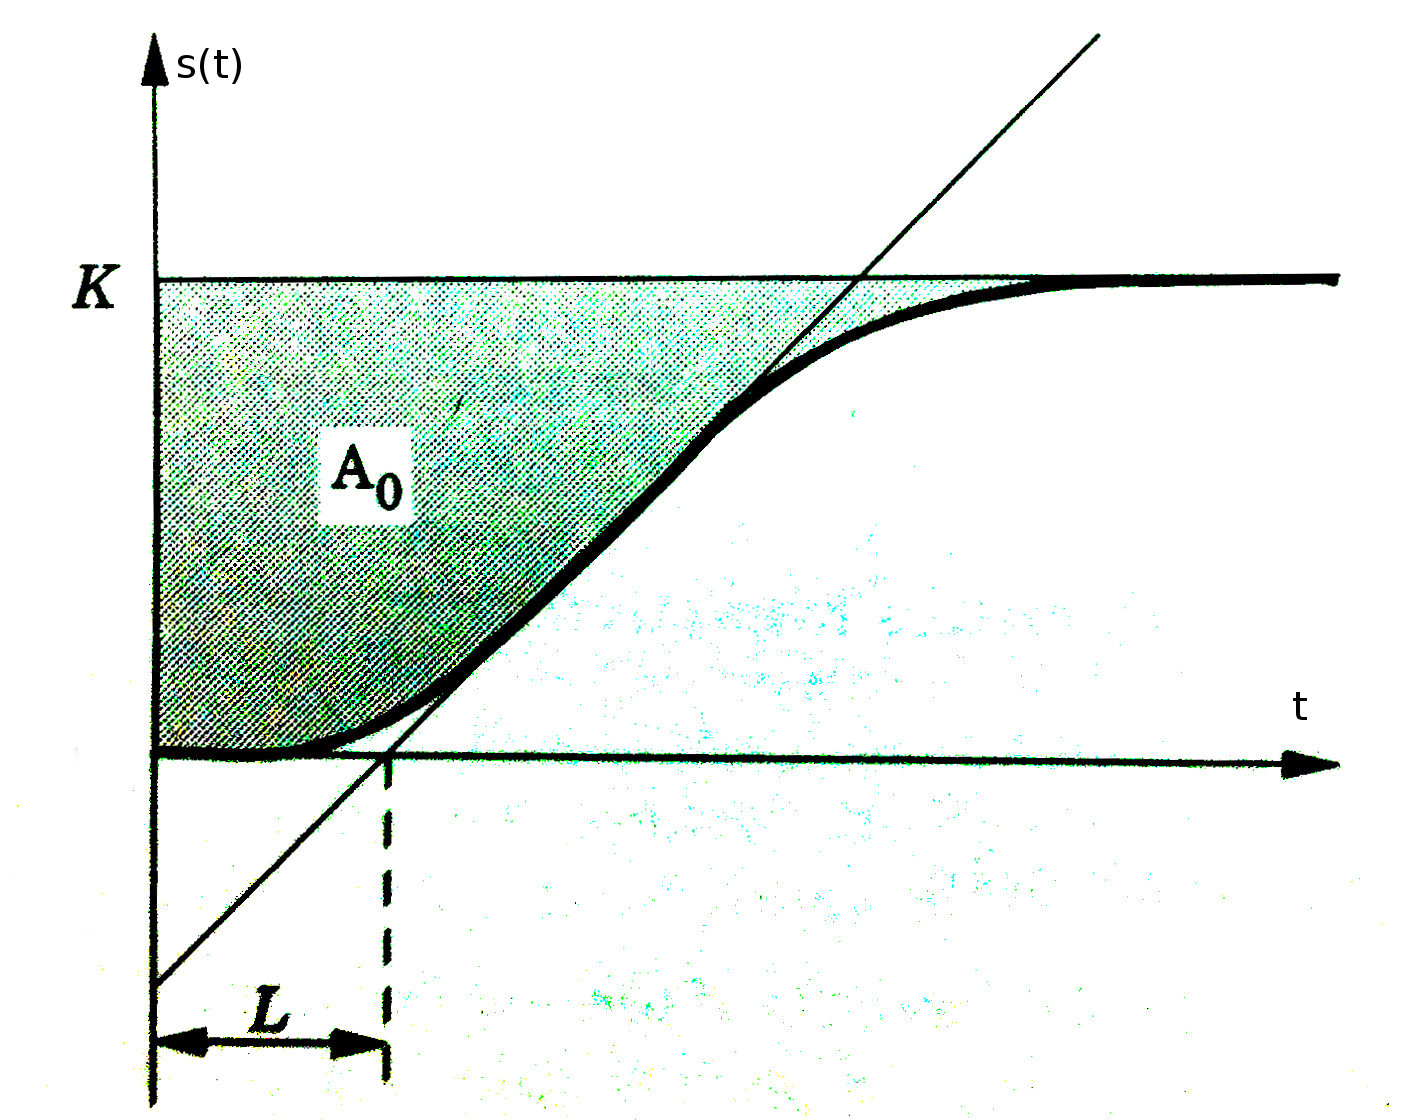
\includegraphics[scale=0.27]{./imagens/resp_g3}
\caption[Gráfico da resposta característica de um processo representado pela equação \ref{eq:g_de_s_3param}]{Gráfico da resposta característica de um processo representado pela equação \ref{eq:g_de_s_3param} \cite{astrom}}
\label{fig:resp_g_de_s_3param}
\end{figure}

A equação a seguir representa curva s(t) apresentada na figura \ref{fig:resp_g_de_s_3param}:

\begin{equation}
s(t) = K(1 - e^{-(t-L)/\tau}) \label{g_de_t_2param}
\end{equation}

Os parâmetros apresentados na equação \ref{eq:g_de_s_3param} podem ser obtidos graficamente. O parâmetro L \textit{(tempo morto)} pode ser obtido interceptando a tangente da resposta do processo no momento de subida ao eixo horizontal, como pode ser visto na figura \ref{fig:resp_g_de_s_3param}. O ganho estático do sistema \textit{(K)} é representado pelo valor final da saída do processo. O valor de $\tau$ pode ser obtido com o auxílio das equações a seguir \cite{astrom}:

\begin{equation}
T = \frac{\int^{+\infty}_0 (s(\infty) - s(t))dt}{K} \label{eq:tau_g_de_s_3param_1}
\end{equation}

\begin{equation}
\tau = T - L \label{eq:tau_g_de_s_3param_2}
\end{equation}

De acordo com \citeonline{astrom}, curvas de respostas à entrada degrau semelhante à apresentada na figura \ref{fig:resp_g_de_s_3param}, caso apresenta um formato "S" \ acentuado, podem ser modeladas pela seguinte equação:

\begin{equation}
G(s) = \frac{K}{(1 + s\tau)^2}e^{-sL} \label{eq:g_de_s_3param_2}
\end{equation}

Sendo a sua resposta no domínio temporal:

\begin{equation}
s(t) = K(1- (1 + \frac{t-L}{\tau})e^{-(t-L)/\tau}) \label{eq:g_de_t_3param_2}
\end{equation}

Nesta formato, o parâmetro $\tau$ pode ser obtido a partir de soluções numéricas.

\subsection{MODELO A QUATRO PARÂMETROS}

De acordo com \citeonline{astrom}, uma aproximação ainda melhor de um processo real pode ser obtido pela seguinte função de transferência:

\begin{equation}
G(s) = \frac{K}{(1 + s\tau_{1})(1 + s\tau_{2})}e^{-sL} \label{eq:g_de_s_4param}
\end{equation}

Este modelo apresenta quatro parâmetros: ganho \textit{(K)}, tempo morto \textit{(L)} e constantes de tempo \textit{($\tau_{1}$ e $\tau_{2}$)}. O ganho e o tempo morto podem ser determinados da mesma forma que foram obtidos no modelo a três parâmetros. No entanto, o cálculo das constantes de tempo envolve solução de equações transcedentes e deve ser encontradas numericamente.

A resposta temporal da equação \ref{eq:g_de_s_4param} quando excitada pelo degrau é:

\begin{equation}
s(t) = K(1 + \frac{\tau_{2}e^{-(t-L)/\tau_{2}} - \tau_{1}e^{-(t-L)/\tau_{1}}}{\tau_{1} - \tau_{2}})
\qquad \tau_{1} \neq \tau_{2} \label{eq:g_de_t_4param}
\end{equation}

% % % % % % % % % % % % % % % % % % % % % % % % % % % % % % % % % % % % % % % % % % % % % % % % % % % % % % % % % % % % % % % % % % % % % % % % % % % % % % % % % % % % % % % % % % % % % % % % % % % % % % % % % % % % % % % % % % % % % % % % % % %

\chapter{CONTROLE DE SISTEMAS DE MALHA FECHADA}

Em função da necessidade de que o robô IRoS cumpra seus movimentos dentro da especificação desejada, é indispensável a realização do projeto de um sistema de  controle em malha fechada para o sistema de manipulação. Esse sistema de controle visa garantir que a posição das juntas tenham precisão em relação ao setpoint fornecido.

\begin{citacao}
"Os sistemas de controle com realimentação são, com frequência, denominados também \textit{sistemas de controle de malha fechada}. Na prática, os termos controle com realimentação e controle de malha fechada são usados indistintamente. Em um sistema de controle de malha fechada, o sinal de erro atuante, que é a diferença entre o sinal de entrada e o sinal de realimentação (que pode ser o próprio sinal de saída ou uma função do sinal de saída e suas derivadas e/ou integrais), realimenta o controlador, de modo que minimize o erro e acerte a saída do sistema ao valor desejado. O termo 'controle de malha fechada' sempre implica a utilização do controle com realimentação para efeito de reduzir o erro do sistema" \cite{ogata}.
\end{citacao}

Normalmente os sistemas de controle são representados por \textit{diagrama de blocos}, descrevendo as inter-relações entre os componentes do processo e indicando o fluxo de sinais do sistema real. O bloco representa uma operação matemática, sendo a função de transferência normalmente incluída nos blocos correspondentes. Desta forma, contém informações relacionadas ao comportamento dinâmico, mas não apresenta informações físicas \cite{ogata}.

Os controladores em malha fechada comparam o valor real da saída da planta com a entrada de referência, buscando reduzir ou zerar este sinal de comparação. A figura \ref{fig:cont_autom} é um diagrama de um sistema de controle, o qual contem um controlador automático, um atuador, uma planta e um sensor \cite{ogata}.

\begin{figure}[h] % Poderia ser \begin{figure}[posicionamento], onde o posicionamento pode ser h - no local do texto onde foi  o comando, t - no topo da pagina atual ou b - no final da pagina de trabalho.
\centering
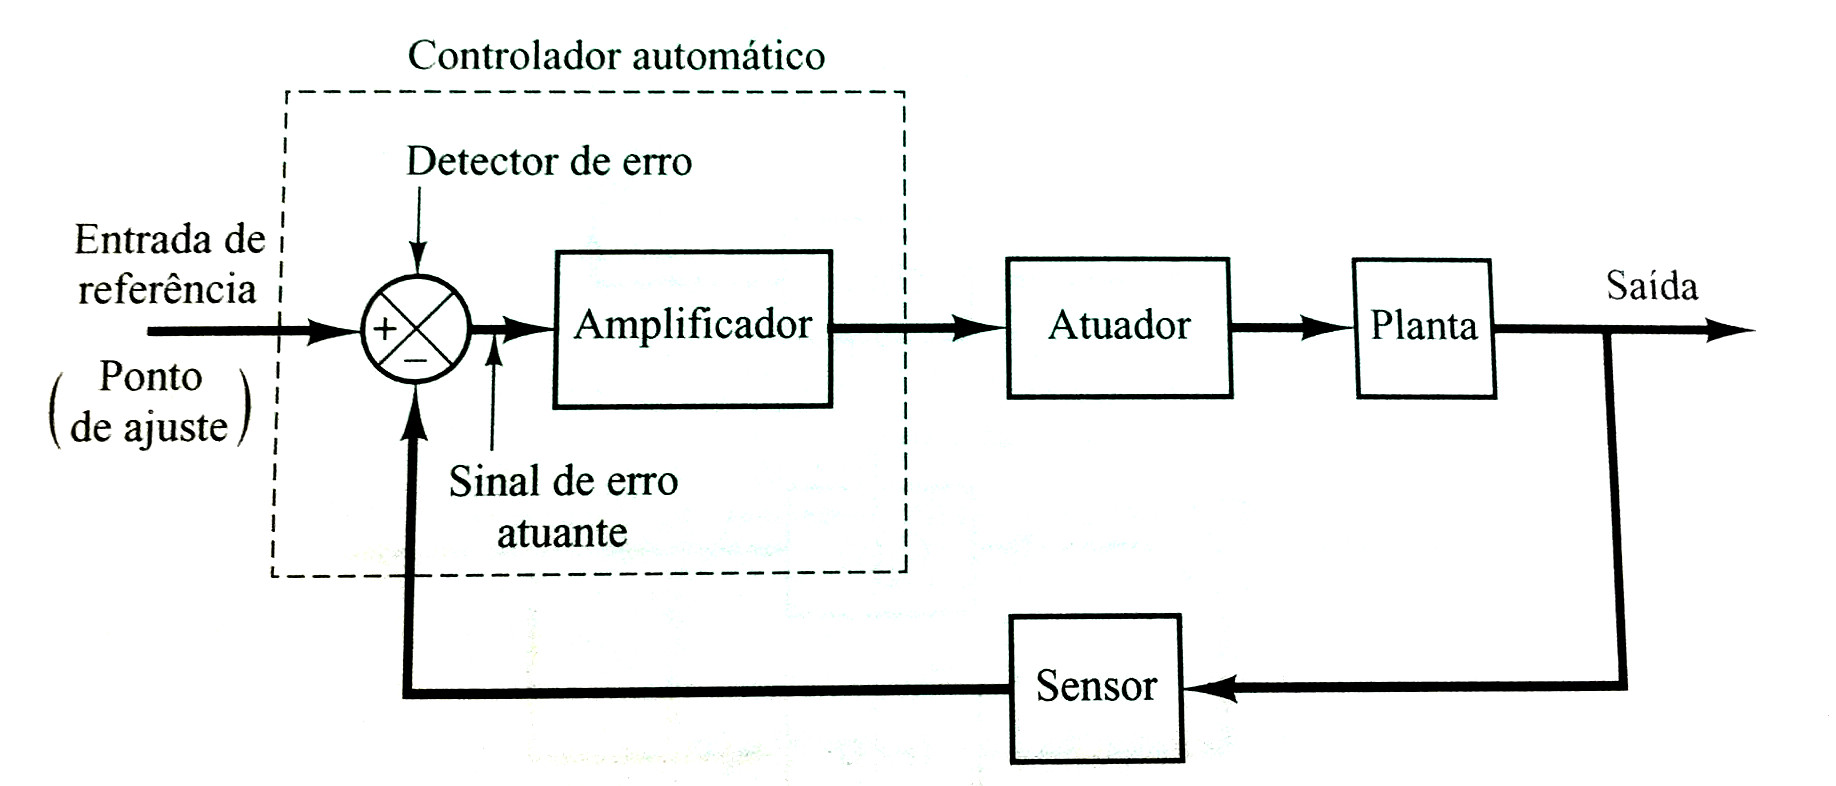
\includegraphics[scale=0.24]{./imagens/cont_autom}
\caption[Diagrama de blocos de um sistema de controle]{Diagrama de blocos de um sistema de controle \cite{ogata}}
\label{fig:cont_autom}
\end{figure}


\section{AÇÕES DE CONTROLE}

Conforme \citeonline{ogata}, os controladores industriais podem ser classificados de acordo com suas ações de controle da seguinte forma:

\begin{enumerate}

\item Controladores on-off;

\item Controladores proporcionais;

\item Controladores integrais;

\item Controladores proporcional-integrais;

\item Controladores proporcional-derivativos;

\item Controladores proporcionais-integral-derivativos.

\end{enumerate}

\subsection{AÇÃO DE CONTROLE ON-OFF}

O controlador on-off é uma estrutura funcional simples, a qual não tem parâmetro a ser configurado e tem apenas duas posições fixas. Esta estratégia busca manter o valor da variável do processo  próximo ao valor de \textit{setpoint}, no entanto, o sistema normalmente apresenta oscilações em relação ao valor de referência \cite{astrom}.

Considerando que o sinal de saída do controlador é u(t) e o sinal de erro atuante é e(t), o controlador on-off é condicionado pela seguinte equação:

\begin{displaymath}
u(t) = \left\{ \begin{array}{ll}
U_{1} & \textrm{para $e(t)>0$}\\
U_{2} & \textrm{para $e(t)<0$}
\end{array} \right.
\end{displaymath}

\subsection{AÇÃO DE CONTROLE PROPORCIONAL}

O controlador de ação proporcional tem a seguinte relação entre a sua saída u(t) e sua entrada \textit{(sinal de erro atuante)} e(t) \cite{ogata}:

$$u(t) = K_{p} e(t)$$

Aplicando a transformada de Laplace na equação anterior, temos:

\begin{equation}
\frac{U(s)}{E(s)} = K_{p} \label{eq:g_s_cont_prop}
\end{equation}

Esta ação de controle pode evitar os problemas de variação do valor da variável do processo, visto que pequenos sinais de controle são gerados para pequenos sinais de erro. No entanto, normalmente pode haver um erro em estado permanente.

\subsection{AÇÃO DE CONTROLE INTEGRAL}

O controlador de ação integral tem a seguinte relação entre a sua saída u(t) e sua entrada \textit{(sinal de erro atuante)} e(t) \cite{ogata}:

$$u(t) = K_{i} \int^{t}_0 e(t)dt$$

Aplicando a transformada de Laplace na equação anterior e considerando as condições iniciais nulas, temos:

\begin{equation}
\frac{U(s)}{E(s)} = \frac{K_{i}}{s} \label{eq:g_s_cont_integ}
\end{equation}

A função principal da ação de controle integral é assegurar que a saída do processo esteja no valor informado pelo setpoint durante o regime permanente. Com a ação de controle integral, um pequeno erro positivo deixará o sinal de controle cada vez maior, e um erro negativo diminuirá o sinal de controle, não importa o quão pequeno é o erro \cite{astrom}.

\subsection{AÇÃO DE CONTROLE PROPORCIONAL-INTEGRAL}

O controlador de ação proporcional-integral tem a seguinte relação entre a sua saída u(t) e sua entrada \textit{(sinal de erro atuante)} e(t) \cite{ogata}:

$$u(t) = K_{p}e(t) + K_{i} \int^{t}_0 e(t)dt$$

Aplicando a transformada de Laplace na equação anterior e considerando as condições iniciais nulas, temos:

\begin{equation}
\frac{U(s)}{E(s)} = K_{p} + \frac{K_{i}}{s} \label{eq:g_s_cont_prop_integ}
\end{equation}

\subsection{AÇÃO DE CONTROLE PROPORCIONAL-DERIVATIVO}

O controlador de ação proporcional-derivativo tem a seguinte relação entre a sua saída u(t) e sua entrada \textit{(sinal de erro atuante)} e(t) \cite{ogata}:

$$u(t) = K_{p}e(t) + K_{d}\frac{de(t)}{dt}$$

Aplicando a transformada de Laplace na equação anterior e considerando as condições iniciais nulas, temos:

\begin{equation}
\frac{U(s)}{E(s)} = K_{p} + K_{d}s \label{eq:g_s_cont_prop_deriv}
\end{equation}

\subsection{AÇÃO DE CONTROLE PROPORCIONAL-INTEGRAL-DERIVATIVO}

O controlador de ação proporcional-integral-derivativo tem a seguinte relação entre a sua saída u(t) e sua entrada \textit{(sinal de erro atuante)} e(t) \cite{ogata}:

$$u(t) = K_{p}e(t) + K_{i} \int^{t}_0 e(t)dt + K_{d}\frac{de(t)}{dt}$$

Aplicando a transformada de Laplace na equação anterior e considerando as condições iniciais nulas, temos:

\begin{equation}
\frac{U(s)}{E(s)} = K_{p} + \frac{K_{i}}{s} + K_{d}s \label{eq:g_s_cont_prop_integ_deriv}
\end{equation}

\section{CONTROLE EM CASCATA}

Normalmente os sistemas de controle são mais complexos que sistemas com uma entrada e uma saída. Logo, um problema a ser resolvido é a escolha das variáveis do processo que devem ser controladas. Dessa forma, o controle em cascata é uma forma de usar vários sinais medidos em uma malha de controle \cite{astrom}.

Um exemplo de controle em cascata pode ser visto na figura \ref{fig:cont_cascata}, onde a malha interna é chamado de malha escrava ou secundário e a malha externa é chamada de malha mestre ou primária. Esta estratégia pode ser usada quando um controle mais rigoroso é necessário, então, pode ser conseguida por meio de um sinal de medição intermédia que responde mais rápido ao sinal de controle \cite{astrom}.

\begin{figure}[h] % Poderia ser \begin{figure}[posicionamento], onde o posicionamento pode ser h - no local do texto onde foi  o comando, t - no topo da pagina atual ou b - no final da pagina de trabalho.
\centering
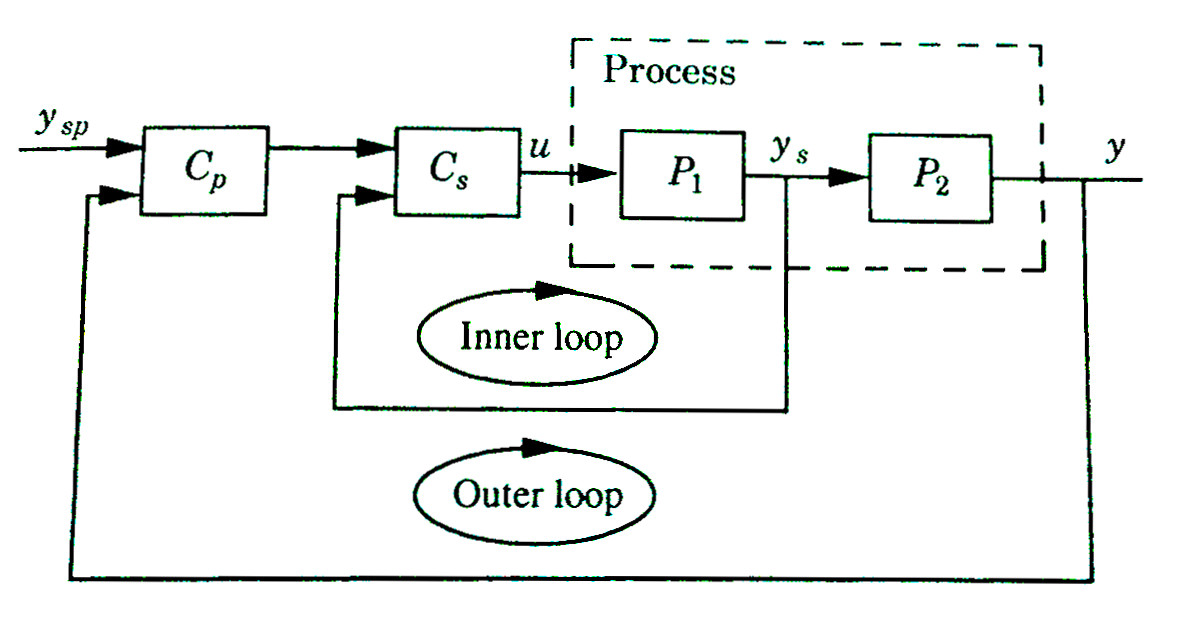
\includegraphics[scale=0.32]{./imagens/cont_casct}
\caption[Diagrama de blocos de um sistema com controladores em cascata]{Diagrama de blocos de um sistema com controladores em cascata \cite{astrom}}
\label{fig:cont_cascata}
\end{figure}

Quando o controladores em cascata são usados, a malha de controle interno detecta distúrbios muito mais rápido que a malha de controle externa. Dessa forma, grande parte das pertubações são eliminadas pelo controlador secundário \cite{astrom}.

%Confirma essa parte do texto com TITO
De acordo com \citeonline{astrom}, para realizar o controle de servomotores pode-se usar controladores em cascata. Sendo que a malha interna ou secundária controlaria a velocidade do servomotor, enquanto a malha externa seria responsável pelo controle de posição. Uma vez que a relação entre posição e velocidade é a integral no tempo, não existe razão para introduzir a ação integral no controle de velocidade nem a ação derivada no controle de posição.

\section{ANÁLISE DO LUGAR DAS RAÍZES}

Sabendo que a resposta transitória do sistema varia de acordo com a localização dos pólos de malha fechada e que pode mudar a depender do parâmetros configurados no controlador, é importante que o projetista saiba como como os pólos da FTMF se movem no plano \textit{s} \cite{ogata}.

O método do lugar das raízes, desenvolvido por W.R. Evans, permite que obter a localização dos pólos da FTMF a partir da variação do ganho do controlador \cite{ogata}.

Considerando o seguinte sistema:

\begin{figure}[h] % Poderia ser \begin{figure}[posicionamento], onde o posicionamento pode ser h - no local do texto onde foi  o comando, t - no topo da pagina atual ou b - no final da pagina de trabalho.
\centering
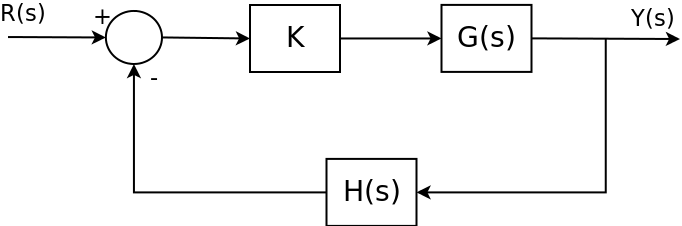
\includegraphics[scale=0.45]{./imagens/Malha_fechada2}
\caption[Diagrama de blocos de um sistema em malha fechada]{Diagrama de blocos de um sistema em malha fechada}
\label{fig:malha_fechada2}
\end{figure}

A função de transferência que relaciona a entrada R(s) com a saída Y(s) será:

\begin{equation}
\frac{Y(s)}{R(s)} = \frac{KG(s)}{1 + KG(s)H(s)} \label{eq:g_s_malha_fechada}
\end{equation}

A equação característica do sistema será:

$$ 1 + KG(s)H(s) = 0 $$

\begin{equation}
KG(s)H(s) = -1 \label{eq:caract}
\end{equation}

A partir da equação \ref{eq:caract} pode-se obter as seguintes condições de módulo e fase:

\begin{itemize}
\item Condição de módulo:

\begin{equation}
|KG(s)H(s)| = 1 \label{eq:cond_mod}
\end{equation}

\item Condição de fase:

\begin{equation}
\phase{KG(s)H(s)} = \pm180^\circ(2k + 1) \qquad (k = 0, 1, 2,...)
\end{equation}

\end{itemize}

Segundo \citeonline{ogata}, o lugar das raízes é o método para localizar a posição das raízes da equação característica do sistema de malha fechada quando um parâmetro específico (normalmente o ganho \textit{K}) varia. Esse gráfico mostra as contribuições de cada pólo ou zero de malha aberta nas localizações dos pólos de malha fechada.

\chapter{SIMULAÇÕES E RESULTADOS EXPERIMENTAIS}

A fim de projetar o sistema de controle de posição do robô, realizou-se a modelagem e o controle de velocidade do servomotor Dynamixel MX-106R em cascata com o controle de posição das juntas que compõem o sistema de manipulação do robô IRoS. A seção \ref{sec:mot_dyn} apresenta mais detalhes sobre o servomotor Dynamixel MX-106R, sua modelagem e seu controle de velocidade. A seção \ref{sec:rob_cemig} exibe maiores particularidades sobre a modelagem e desenvolvimento do sistema de controle de posição das juntas do robô.

\section{MOTOR DYNAMIXEL MX-106R} \label{sec:mot_dyn}

O servomotor Dynamixel MX-106R foi selecionado para realizar o movimento das juntas do robô através de uma criteriosa análise. Levou-se em consideração nesta análise: a massa, os requisitos de torque necessário, a dimensão, a tensão de alimentação e a velocidade \cite{cemig}.

\begin{figure}[h] % Poderia ser \begin{figure}[posicionamento], onde o posicionamento pode ser h - no local do texto onde foi  o comando, t - no topo da pagina atual ou b - no final da pagina de trabalho.
\centering
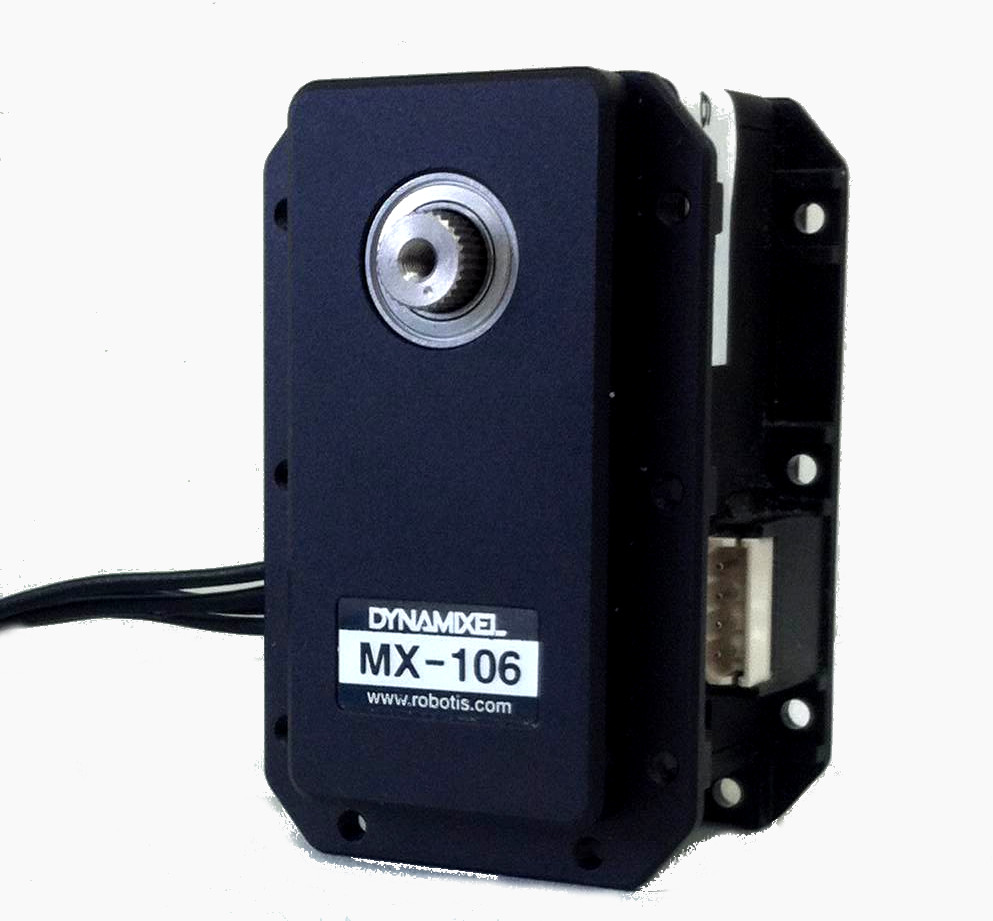
\includegraphics[scale=0.32]{./imagens/MX-106R}
\caption[Motor Dynamixel MX-106R]{Motor Dynamixel MX-106R}
\label{fig:mx-106r}
\end{figure}

Algumas das características do servomotor MX-106R ilustrado na figura \ref{fig:mx-106r} são \cite{cemig}:

\begin{itemize}

\item Comunicação digital através de interface em rede RS-485;

\item Amplitude de rotação de $360^\circ$ e capacidade de giro contínuo;

\item Controlador PID com parâmetros configuráveis;

\item Encoder magnético absoluto com resolução de 12 bits.

\end{itemize}

De acordo com \citeonline{cemig}, os servomotores Dynamixel MX-106R serão controlados a partir do ROS, utilizando-se interface de comunicação serial.

\subsection{MODELAGEM DO MOTOR DYNAMIXEL MX-106R}

Com o propósito de obter o modelo matemático do servomotor Dynamixel MX-106R, realizou-se uma série de ensaios experimentais. Os ensaios tem a finalidade de auxiliar na modelagem matemática e em obter a transformada de Laplace da relação entre os sinais de saída e entrada do servomotor. Dessa forma, pode-se conseguir a função de transferência do servomotor e posteriormente aplicar ações de controle PID no sistema.

Os ensaios experimentais foram realizados seguindo quase todos os métodos indicados na seção \ref{sec:mod_degrau} deste documento \cite{astrom}. No entanto, o servomotor Dynamixel MX-106R apresenta uma malha de controle interna, impossibilitando a realização do ensaio em malha aberta. Então optou-se pela execução do experimento em malha fechada, mas atribuindo valor igual a zero aos ganhos integral e derivativo no controlador interno ao MX-106R. Usou-se apenas o ganho proporcional do controlador com valor diferente de zero. Desta forma, foi estimado uma função de transferência em malha aberta para o servomotor a partir de uma função de transferência em malha fechada inicialmente calculada.

Conforme \citeonline{astrom}, ensaios experimentais para obtenção de modelos devem ser repetidos variando a amplitude do sinal de entrada e as condições de operação. Visando atender esta recomendação, os seguintes parâmetros foram modificados a cada experimento, buscando-se também verificar a linearidade entre as diferentes regiões de operação do servomotor:

\begin{itemize}

\item Velocidade de operação \textit{(sinal de entrada do servomotor)};

\item Torque solicitado;

\item Ganho proporcional do controlador interno ao servomotor Dynamixel MX-106R;

\end{itemize}

De acordo com \citeonline{ogata}, um sistema é linear caso possa se aplicar o princípio da superposição. "Na pesquisa experimental de um sistema dinâmico, se causa e efeito forem proporcionais, significando assim que é válida a aplicação do princípio da superposição, então o sistema pode ser considerado linear".

Realizou-se cinco ensaios experimentais. O sistema equivalente ao testado pode ser observado na figura \ref{fig:malha_fechada2} e as características e resultados de cada um dos ensaios foram:\\

\begin{itemize}

\item Ensaio 1:
 
r(t) = $\pm$1 rad/s;\\
torque = 2 N.m;\\
Kp = 1.\\
\\
\\

\begin{figure}[h] % Poderia ser \begin{figure}[posicionamento], onde o posicionamento pode ser h - no local do texto onde foi  o comando, t - no topo da pagina atual ou b - no final da pagina de trabalho.
\centering
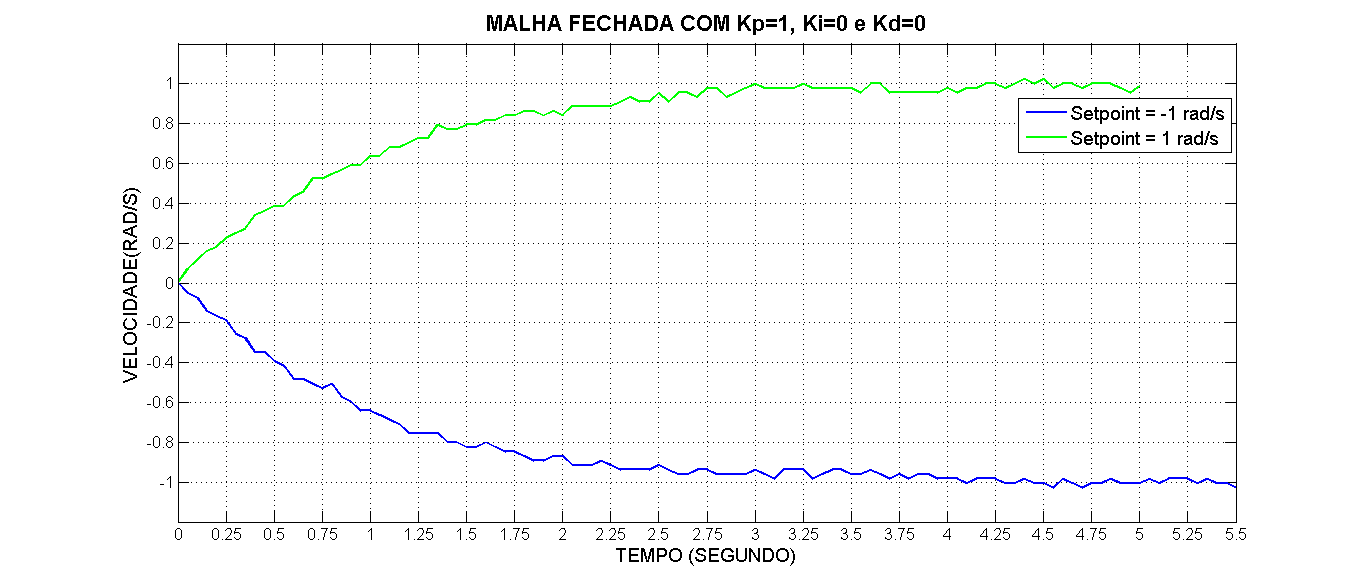
\includegraphics[scale=0.48]{./imagens/Ensaio1}
\caption[Ensaio Experimental 1: Motor Dynamixel MX-106R]{Ensaio Experimental 1: Motor Dynamixel MX-106R}
\label{fig:ensaio1}
\end{figure}


\item Ensaio 2:
 
r(t) = $\pm$1,5 rad/s;\\
torque = 2 N.m;\\
Kp = 1.\\
\\
\\
\\
\\
\\

\begin{figure}[h] % Poderia ser \begin{figure}[posicionamento], onde o posicionamento pode ser h - no local do texto onde foi  o comando, t - no topo da pagina atual ou b - no final da pagina de trabalho.
\centering
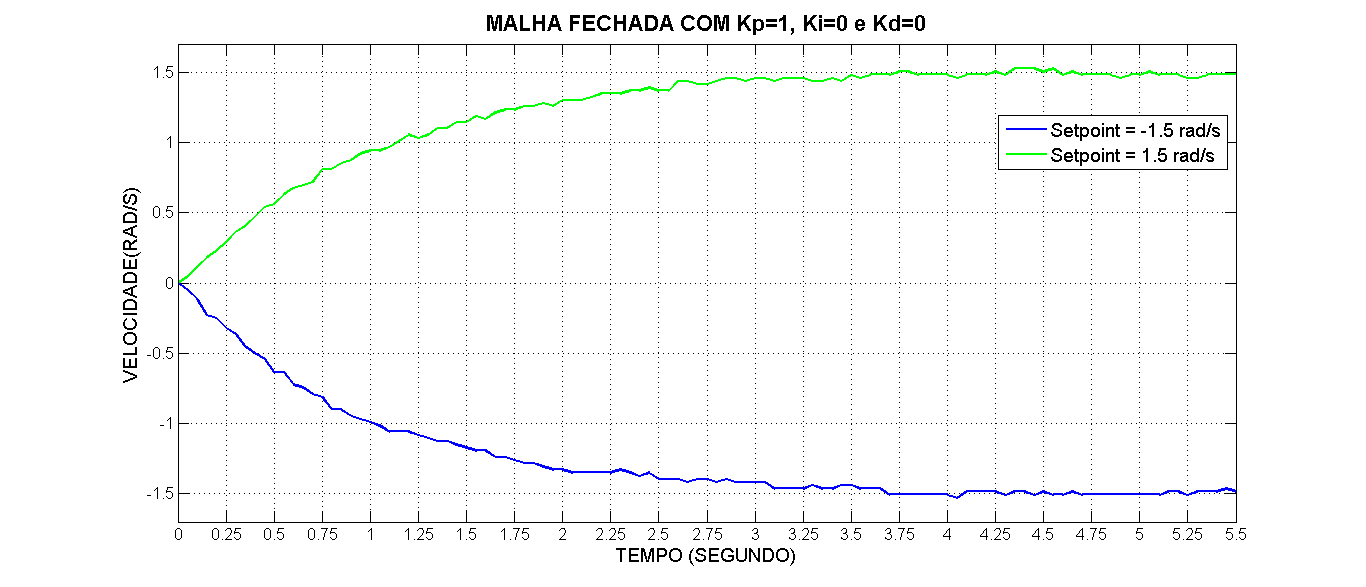
\includegraphics[scale=0.48]{./imagens/Ensaio2}
\caption[Ensaio Experimental 2: Motor Dynamixel MX-106R]{Ensaio Experimental 2: Motor Dynamixel MX-106R}
\label{fig:ensaio2}

\end{figure}

\item Ensaio 3:
 
r(t) = $\pm$1 rad/s;\\
torque = 2 N.m;\\
Kp = 5.\\
\\
\\

\begin{figure}[h] % Poderia ser \begin{figure}[posicionamento], onde o posicionamento pode ser h - no local do texto onde foi  o comando, t - no topo da pagina atual ou b - no final da pagina de trabalho.
\centering
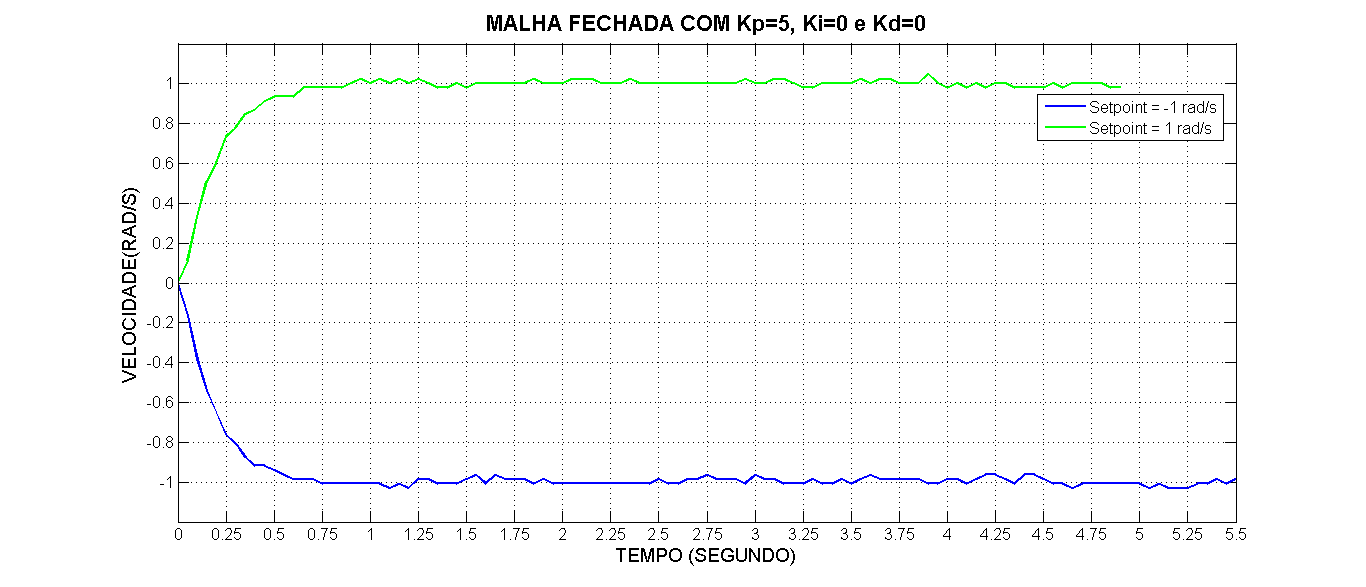
\includegraphics[scale=0.48]{./imagens/Ensaio3}
\caption[Ensaio Experimental 3: Motor Dynamixel MX-106R]{Ensaio Experimental 3: Motor Dynamixel MX-106R}
\label{fig:ensaio3}
\end{figure}

\item Ensaio 4:
 
r(t) = $\pm$1 rad/s;\\
torque = 3 N.m;\\
Kp = 1.\\

\begin{figure}[h] % Poderia ser \begin{figure}[posicionamento], onde o posicionamento pode ser h - no local do texto onde foi  o comando, t - no topo da pagina atual ou b - no final da pagina de trabalho.
\centering
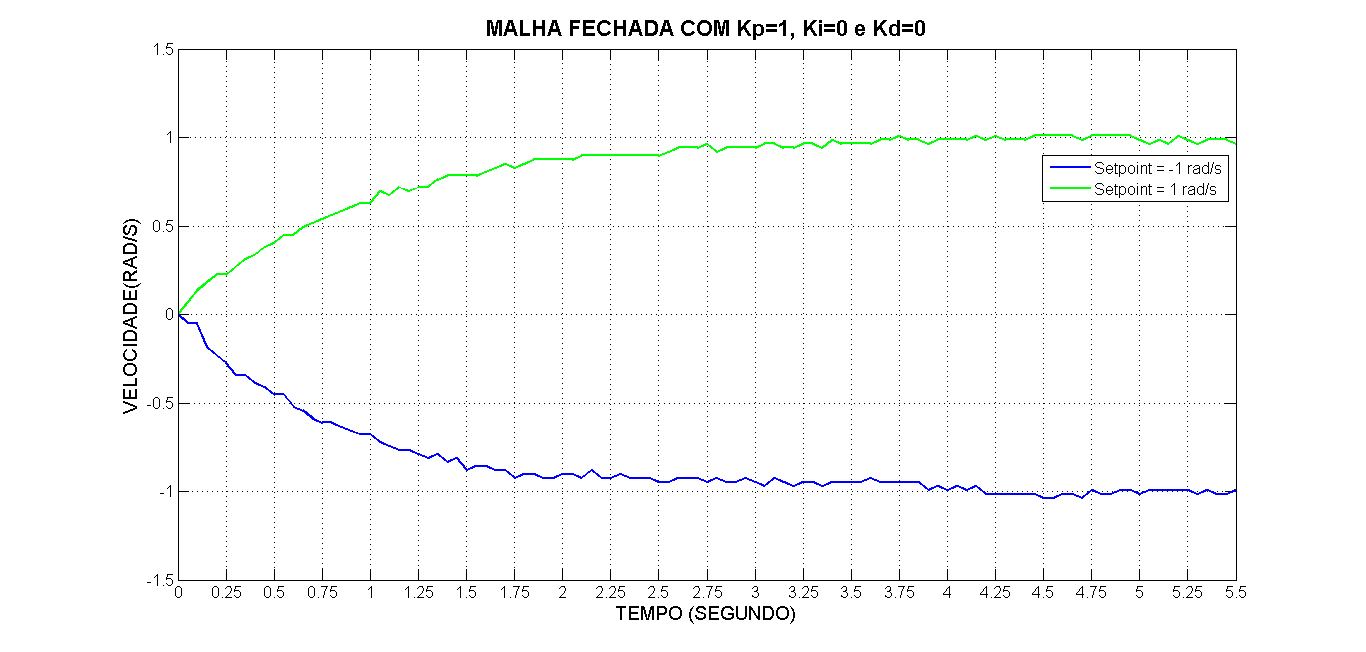
\includegraphics[scale=0.47]{./imagens/Ensaio4}
\caption[Ensaio Experimental 4: Motor Dynamixel MX-106R]{Ensaio Experimental 4: Motor Dynamixel MX-106R}
\label{fig:ensaio4}

\end{figure}

\item Ensaio 5:
 
r(t) = $\pm$1 rad/s;\\
torque = 3 N.m;\\
Kp = 5.

\begin{figure}[h] % Poderia ser \begin{figure}[posicionamento], onde o posicionamento pode ser h - no local do texto onde foi  o comando, t - no topo da pagina atual ou b - no final da pagina de trabalho.
\centering
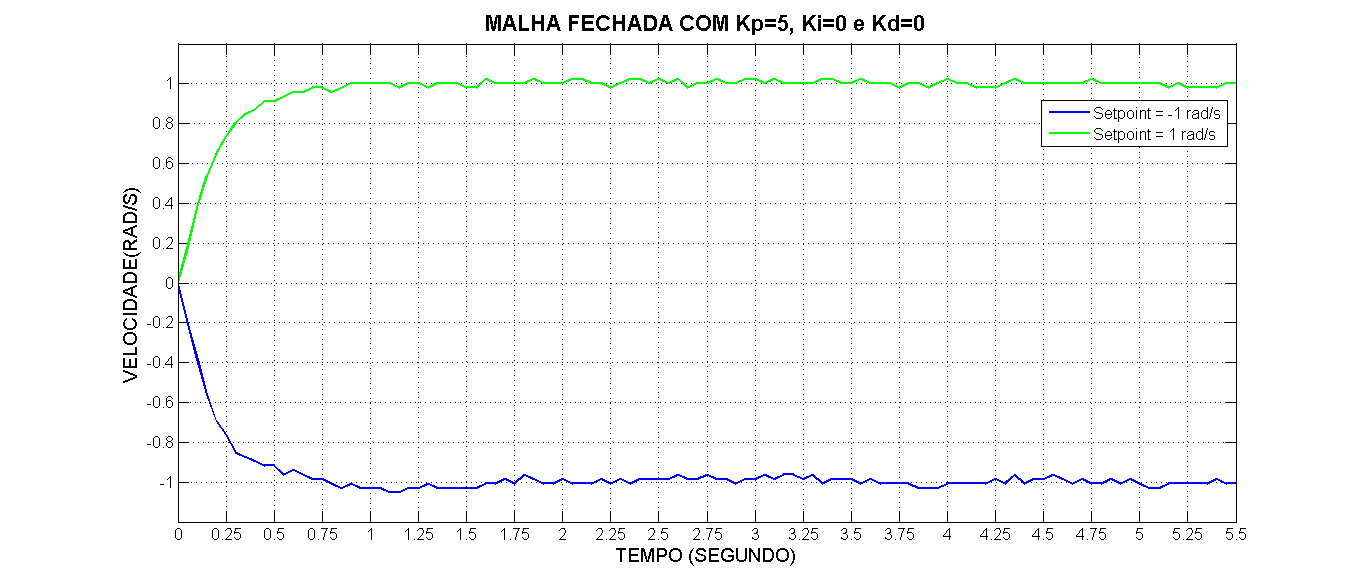
\includegraphics[scale=0.46]{./imagens/Ensaio5}
\caption[Ensaio Experimental 5: Motor Dynamixel MX-106R]{Ensaio Experimental 5: Motor Dynamixel MX-106R}
\label{fig:ensaio5}
\end{figure}

\end{itemize}

Com o propósito de obter um modelo equivalente do sistema em malha fechada, pode-se comparar os resultados apresentados acima com a figura \ref{fig:resp_g_de_s_2param}. Esta comparação permite que o sistema do composto pelo servomotor Dynamixel MX-106R e seu controlador em malha fechada, quando este apresenta apenas o ganho proporcional ativado, seja aproximado por um sistema de primeira ordem. A função de transferência das respostas dos sistemas, cuja as curvas foram apresentadas acima pode ser descrita pela seguinte equação:

\begin{equation}
G(s) = \frac{K}{1 + \tau s} \label{eq:g_s_1_ordem_MF}
\end{equation}

A partir das equações \ref{eq:k_mod_2_param}, \ref{eq:tau_mod_2_param_1} e \ref{eq:tau_mod_2_param_2} e dos conceitos apresentados na seção \ref{sec:mod_2_param}, pode-se calcular os parâmetros K e $\tau$.

A partir da aproximação da FTMF do sistema servomotor-controlador por um sistema de primeira ordem, estimou-se que servomotor em malha aberta pode apresentar dois modelos:

\begin{enumerate}

\item Modelo de primeira ordem:
$G(s) = \frac{K^{'}}{1 + \tau^{'} s}$

\item Modelo integrado:
$G(s) = \frac{K^{'}}{s}$

\end{enumerate}

Os cálculos dos modelos em malha aberta a partir do modelo de malha fechada podem ser observados nas seções \ref{sec:aprox_mod_1_ord} e \ref{sec:aprox_mod_int}.

\subsubsection{APROXIMAÇÃO POR MODELO DE PRIMEIRA ORDEM} \label{sec:aprox_mod_1_ord}

Conforme informado nas seções anteriores, os ensaios foram realizados em um sistema de malha fechada com realimentação unitária \textit{(H(s) = 1)} semelhantes à figura \ref{fig:malha_fechada2}. Logo, sendo o modelo calculado em malha fechada a partir dos experimentos realizados, e exibidos na seção anterior, foi calculado através de uma aproximação uma função de transferência de malha aberta equivalente de primeira ordem.

Considerando que a FTMA, G(s), do servomotor tem o seguinte formato:

$$G(s) = \frac{K^{'}}{1 + \tau^{'} s}$$

Logo, a FTMF, controlador C(s)-servomotor G(s), com realimentação unitária será:

$$G(s) = \frac{C(s)G(s)}{1 + C(s)G(s)} = \frac{\frac{K^{'} K_{p}}{1 + \tau^{'} s}}{1 + \frac{K^{'} K_{p}}{1 + \tau^{'} s}} = \frac{K^{'} K_{p}}{1 + K^{'} K_{p} + \tau^{'} s}$$
\\
\begin{equation}
G(s) = \frac{\frac{K^{'} K_{p}}{K^{'} K_{p} + 1}}{1 + \frac{\tau^{'}}{K^{'} K_{p} + 1} s} \label{eq:g_s_MA_para_MF} \qquad Sendo \ C(s) = K_{p}
\end{equation}

Comparando a equação \ref{eq:g_s_MA_para_MF} com a equação \ref{eq:g_s_1_ordem_MF} temos:

$$\frac{K^{'} K_{p}}{K^{'} K_{p} + 1} = K$$

\begin{equation}
K^{'} = \frac{K}{K_{p} - K K_{p}} \label{eq:k_linha}
\end{equation}

$$ \frac{\tau^{'}}{K^{'} K_{p} + 1} = \tau$$

\begin{equation}
\tau^{'} = \tau (K^{'} K_{p} + 1) \label{eq: tau_linha}
\end{equation}

A partir das equações \ref{eq:k_linha} e \ref{eq: tau_linha} pode obter uma aproximação de primeira ordem do modelo em malha aberta do servomotor Dynamixel MX-106R. O modelo de primeira ordem em malha aberta calculado a partir dos ensaios experimentais pode ser representado a partir da seguinte equação:

$$G(s) = \frac{452,1}{1 + 451,8 s}$$

\subsubsection{APROXIMAÇÃO POR MODELO INTEGRADOR} \label{sec:aprox_mod_int}

Realizando os mesmos procedimentos da seção anterior, mas considerando que a FTMA, G(s), do servomotor tem o seguinte formato:

$$G(s) = \frac{K^{'}}{s}$$

Logo, a FTMF, controlador C(s)-servomotor G(s), com realimentação unitária será:

$$G(s) = \frac{C(s)G(s)}{1 + C(s)G(s)} = \frac{\frac{K^{'} K_{p}}{s}}{1 + \frac{K^{'} K_{p}}{s}} = \frac{K^{'} K_{p}}{s +  K^{'} K_{p}}$$

\begin{equation}
G(s) = \frac{1}{1 + \frac{1}{K^{'} K_{p}} s} \label{eq:g_s_MA_para_MF_int} \qquad Sendo \ C(s) = K_{p}
\end{equation}

Comparando a equação \ref{eq:g_s_MA_para_MF_int} com a equação \ref{eq:g_s_1_ordem_MF} temos:

$$ \frac{1}{K^{'} K_{p}} = \tau $$

\begin{equation}
K^{'} = \frac{1}{K_{p} \tau}
\end{equation}

Dessa forma, o modelo integrado em malha aberta calculado a partir dos ensaios experimentais pode ser representado a partir da seguinte equação:

$$ G(s) = \frac{1,002}{s} $$

\subsection{SIMULAÇÃO COMPUTACIONAL DO MODELO DO MX-106R}

A partir do cálculo de modelos em malha aberta por uma aproximação de primeira ordem e por uma aproximação integradora, realizou-se simulação computacional no software Matlab buscando reproduzir as mesmas condições dos ensaios experimentais. Dessa forma, utilizou-se a FTMA calcula do servomotor e FT do controlador configurado com o mesmo parâmetro utilizado no experimento.

A figura \ref{fig:malha_fechada2} representa pode representar o diagrama simulado, no qual:

\begin{itemize}

\item G(s) representa a FTMA do servomotor;

\item K representa o ganho proporcional do controlador. Lembrando que o valor deste ganho sofreu variação de acordo com os ensaios do experimento;

\item H(s) = 1 \textit{(realimentação unitária)}.
\\

\end{itemize}

O resultado da simulação computacional do modelo de malha aberta do servomotor Dynamixel MX-106R quando submetido às mesmas condições do ensaio experimental pode ser visto nas figuras a seguir:
\\
\\

\begin{itemize}

\item Ensaio 1:
\\
r(t) = $\pm$1 rad/s;\\
%torque = 2 N.m;\\
Kp = 1.\\
\\

\begin{figure}[h] % Poderia ser \begin{figure}[posicionamento], onde o posicionamento pode ser h - no local do texto onde foi  o comando, t - no topo da pagina atual ou b - no final da pagina de trabalho.
\centering
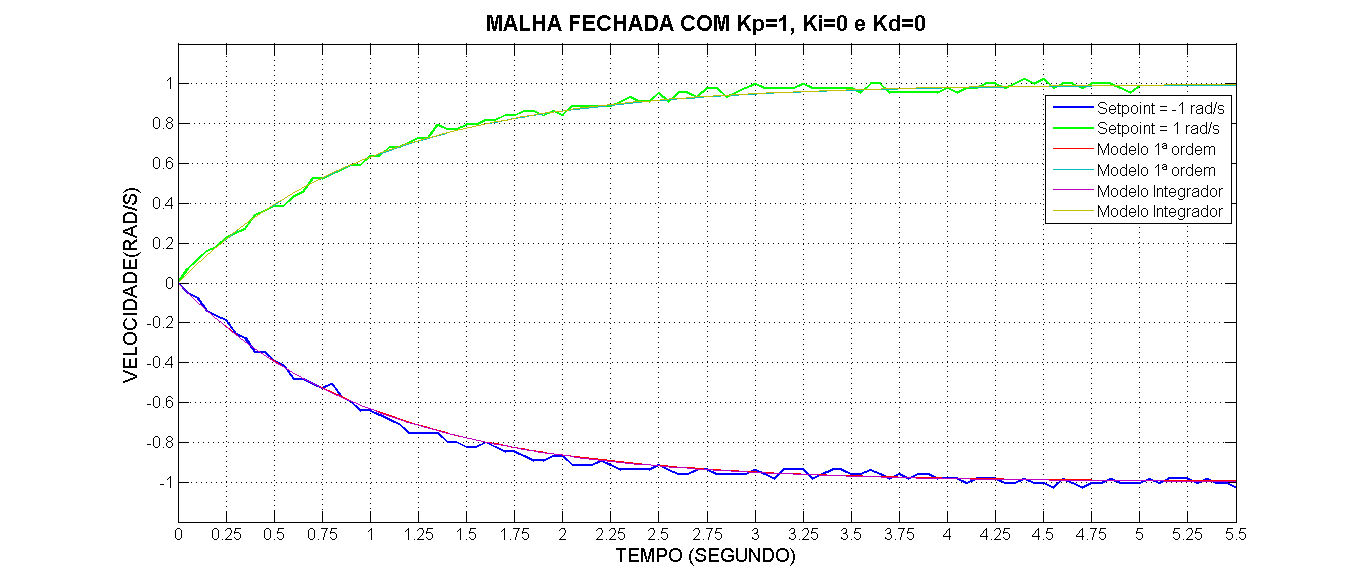
\includegraphics[scale=0.48]{./imagens/Mod_Ensaio1}
\caption[Comparação entre Simulação e Ensaio Experimental 1: Motor Dynamixel MX-106R]{Comparação entre Simulação e Ensaio Experimental 1: Motor Dynamixel MX-106R}
\label{fig:mod_ensaio1}
\end{figure}

\item Ensaio 2:

r(t) = $\pm$1,5 rad/s;\\
%torque = 2 N.m;\\
Kp = 1.\\

\begin{figure}[h] % Poderia ser \begin{figure}[posicionamento], onde o posicionamento pode ser h - no local do texto onde foi  o comando, t - no topo da pagina atual ou b - no final da pagina de trabalho.
\centering
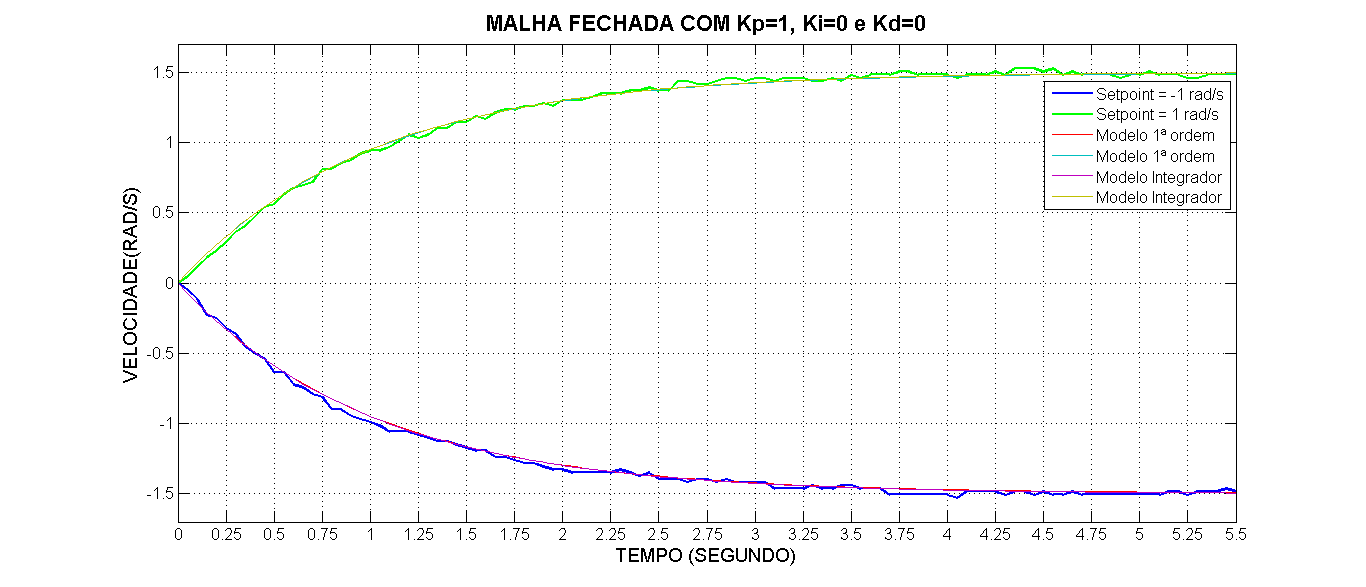
\includegraphics[scale=0.48]{./imagens/Mod_Ensaio2}
\caption[Comparação entre Simulação e Ensaio Experimental 2: Motor Dynamixel MX-106R]{Comparação entre Simulação e Ensaio Experimental 2: Motor Dynamixel MX-106R}
\label{fig:mod_ensaio2}
\end{figure}

\item Ensaio 3:

r(t) = $\pm$1 rad/s;\\
%torque = 2 N.m;\\
Kp = 5.\\

\begin{figure}[h] % Poderia ser \begin{figure}[posicionamento], onde o posicionamento pode ser h - no local do texto onde foi  o comando, t - no topo da pagina atual ou b - no final da pagina de trabalho.
\centering
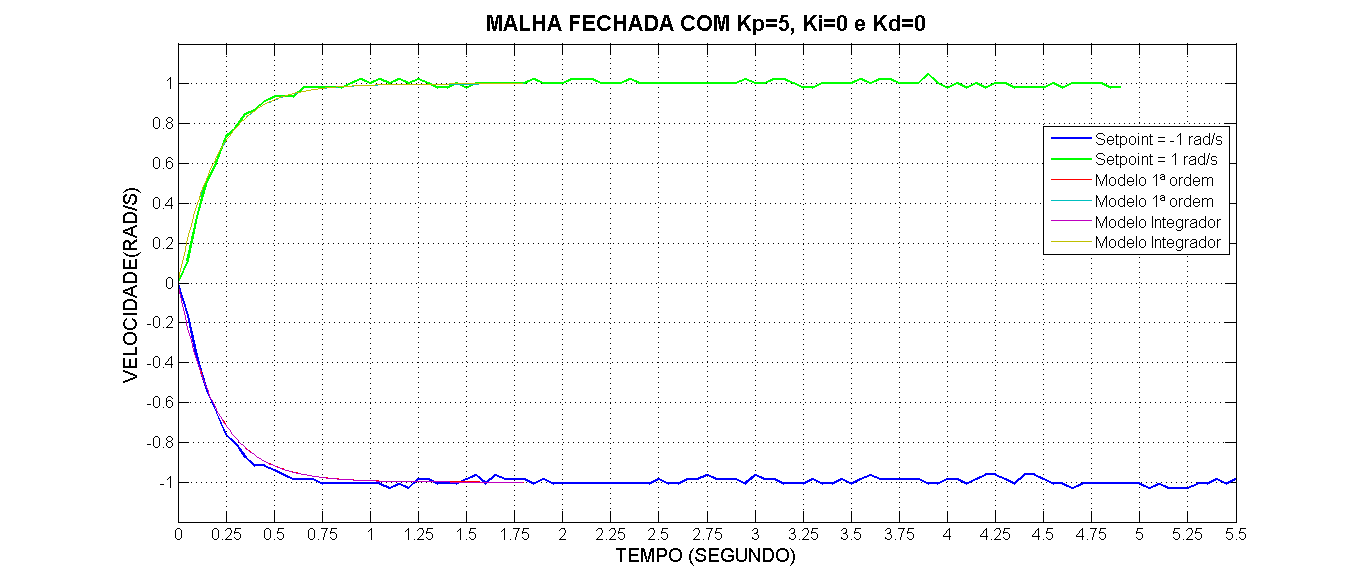
\includegraphics[scale=0.48]{./imagens/Mod_Ensaio3}
\caption[Comparação entre Simulação e Ensaio Experimental 3: Motor Dynamixel MX-106R]{Comparação entre Simulação e Ensaio Experimental 3: Motor Dynamixel MX-106R}
\label{fig:mod_ensaio3}
\end{figure}

\item Ensaio 4:
\\
r(t) = $\pm$1 rad/s;\\
%torque = 3 N.m;\\
Kp = 1.\\
\\

\begin{figure}[h] % Poderia ser \begin{figure}[posicionamento], onde o posicionamento pode ser h - no local do texto onde foi  o comando, t - no topo da pagina atual ou b - no final da pagina de trabalho.
\centering
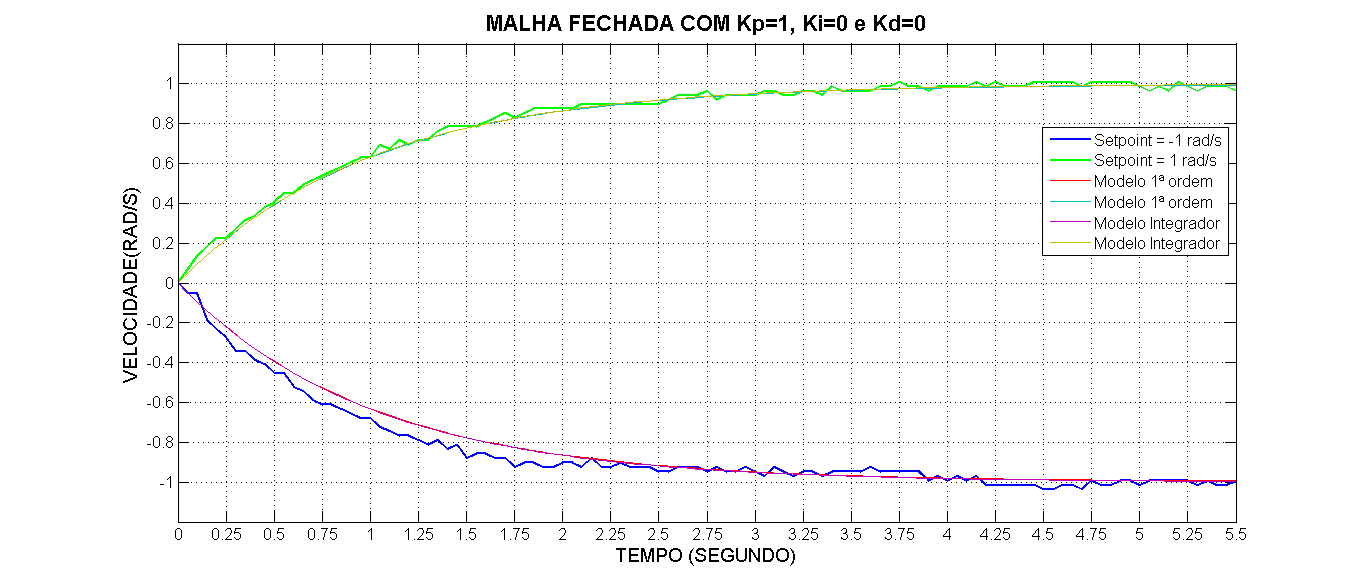
\includegraphics[scale=0.48]{./imagens/Mod_Ensaio4}
\caption[Comparação entre Simulação e Ensaio Experimental 4: Motor Dynamixel MX-106R]{Comparação entre Simulação e Ensaio Experimental 4: Motor Dynamixel MX-106R}
\label{fig:mod_ensaio4}
\end{figure}

\item Ensaio 5:

r(t) = $\pm$1 rad/s;\\
%torque = 3 N.m;\\
Kp = 5.\\

\begin{figure}[h] % Poderia ser \begin{figure}[posicionamento], onde o posicionamento pode ser h - no local do texto onde foi  o comando, t - no topo da pagina atual ou b - no final da pagina de trabalho.
\centering
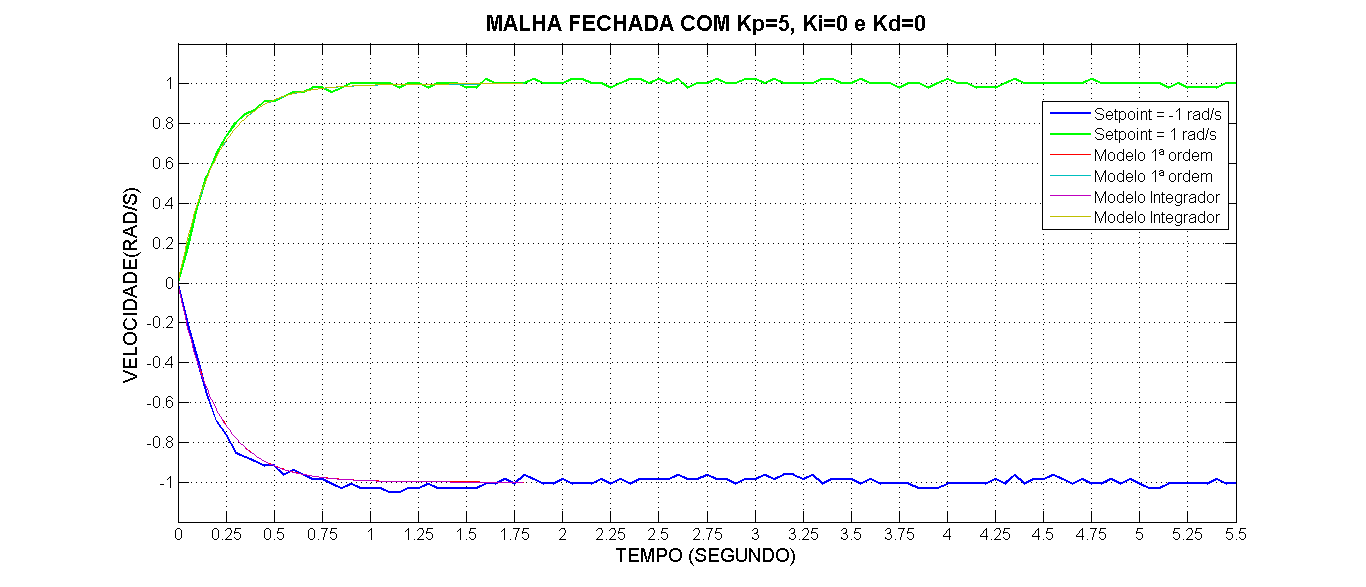
\includegraphics[scale=0.48]{./imagens/Mod_Ensaio5}
\caption[Comparação entre Simulação e Ensaio Experimental 5: Motor Dynamixel MX-106R]{Comparação entre Simulação e Ensaio Experimental 5: Motor Dynamixel MX-106R}
\label{fig:mod_ensaio5}
\end{figure}

\end{itemize}

%PAREI AQUI EXATAMENTE

\subsection{PREJETO DO CONTROLADOR DO MOTOR DYNAMIXEL MX-106R}

%A figura \ref{fig:blocos_clp} representa o diagramas de bloco geral de um CLP. Este equipamento é constituído por dois elementos principais: uma unidade de processamento (CPU) e interfaces de entrada e saída. \cite{silveira}

%As variáveis de entrada são os sinais que chega do mundo externo ao CLP, podem ser provenientes tanto do processo industrial quanto de sinais gerados pelo operador. As variáveis de saída são respostas geradas pelo controlador, podendo ser utilizadas para acionamento de equipamentos ou para sinalização de estados nos painéis. A CPU processa a programação gravada na memória realizando ciclicamente a leitura das entradas, execução do programa e atualização das saídas. Um ciclo destes ocorre na faixa de mili ou microssegundos. \cite{silveira}

%A figura \ref{fig:blocos_clp} representa o diagramas de bloco geral de um CLP. Este equipamento é constituído por dois elementos principais: uma unidade de processamento (CPU) e interfaces de entrada e saída. \cite{silveira}

\subsection{SIMULAÇÃO COMPUTACIONAL DO SISTEMA MOTOR \textit{(MX-106R)} - CONTROLADOR}

%A figura \ref{fig:blocos_clp} representa o diagramas de bloco geral de um CLP. Este equipamento é constituído por dois elementos principais: uma unidade de processamento (CPU) e interfaces de entrada e saída. \cite{silveira}

% % % % % % % % % % % % % % % % % % % % % % % % % % % % % % % % % %

\section{ROBÔ} \label{sec:rob_cemig}

%TEXTO SOBRE O ROBÔ CEMIG

\subsection{MODELAGEM DO ROBÔ CEMIG}

%FALAR SOBRE A FORMA UTILIZADA PARA MODELAR ROBÔ CEMIG

\subsection{SIMULAÇÃO COMPUTACIONAL DO MODELO DO ROBÔ CEMIG}

%FALAR SOBRE A SIMUAÇÃO DO MODELO

\subsection{PREJETO DO CONTROLADOR DO ROBÔ CEMIG}

%A figura \ref{fig:blocos_clp} representa o diagramas de bloco geral de um CLP. Este equipamento é constituído por dois elementos principais: uma unidade de processamento (CPU) e interfaces de entrada e saída. \cite{silveira}

\subsection{SIMULAÇÃO COMPUTACIONAL DO SISTEMA ROBÔ - CONTROLADOR}

%A figura \ref{fig:blocos_clp} representa o diagramas de bloco geral de um CLP. Este equipamento é constituído por dois elementos principais: uma unidade de processamento (CPU) e interfaces de entrada e saída.\cite{ogata}

% % % % % % % % % % % % % % % % % % % % % % % % % % % % % % % % % % % % % % % % % % % % % % % % % % % % % % % % % % % % % % % % % % % % % % % % % % % % % % % % % % % % % % % % % % % % % % % % % % % % % % % % % % % % % % % % % % % % % % % % % % %%

\chapter{CONSIDERAÇÕES FINAIS}

%Os CLPs\footnote{Também conhecidos como PLC, abreviatura do termo em inglês \textit{Programmable Logic Controller}} são equipamentos digitais capazes de controlar máquinas e processos, tornando possível a implementação de uma lógica de programação de forma dinâmica e flexível. É capaz, através de funções simples, realizar energização/desenergização, temporização, contagem, sequenciamento, operações matemáticas e manipulações de dados\cite{moraes}.

%\begin{enumerate}
%\item \textbf{Entendimento do processo}: Consiste num estudo detalhado do processo a ser automatizado. Nesta fase devem ser levantados quais dados devem ser monitorados e historiados. 

%\item \textbf{Tomada de dados}: Nesta etapa são escolhidas quais dados estarão presentes no sistema supervisório, de forma que este se torne conciso, facilitando a visualização e manuseio do sistema. Em situações onde estes dados trafeguem em rede, um grande número de dados pode acarretar em perda de desempenho no tráfego de informação.

%\item \textbf{Planejamento do banco de dados}: Em plantas de maior porte e complexidade é necessário utilizar um banco de dados para tratar as \textit{tags}. Antes de montar o banco de dados é necessário definir qual será a velocidade de leitura das variáveis (\textit{scan}) e criar uma metodologia para nomeação (criação de \textit{tags}) e armazenamento das variáveis.

%\item \textbf{Planejamento dos alarmes}: Esta etapa requer o envolvimento dos responsáveis técnicos pelo processo para definições das condições de acionamento dos alarmes, o modo de notificação ao operador e as ações que devem ser tomadas. É importante levar em conta que um grande número de alarmes pode causar sobrecarga no operador, podendo tornar confusa a operação em momentos agitados. Por isso é necessário que se faça uma filtragem dos alarmes realmente relevantes.

%\item \textbf{Planejamento da navegação entre telas}: A organização das telas do processo em grupos com elementos relacionados (de uma mesma área ou processo, por exemplo) e condizentes com a realidade da planta facilita o uso do sistema, reduzindo o tempo necessário para o aprendizado.

%\item \textbf{Desenho das telas}: Da mesma forma que para o planejamento da navegação, o desenho das telas deve visar simplificar a sua utilização. Além disso, deve se buscar manter um padrão de cores, de nomenclatura e de distribuição dos botões nas telas. Os elementos gráficos do padrão ISA (\textit{International Society of Automation}) são recomendados pois o seu uso é comum na indústria, assim como utilizar cores com significados reconhecidos, como o verde e o vermelho.

%\item \textbf{Gráfico de tendências}: Estes elementos demonstram o comportamento das variáveis analisadas ao longo do tempo. Podem ser utilizados, por exemplo, para analisar tendências, monitorar a qualidade do processo e observar a relação entre variáveis distintas.

%\item \textbf{Planejamento do sistema de segurança}: No desenvolvimento de um sistema supervisório é possível restringir o acesso através de senhas.

%\item \textbf{Padrão Industrial de Desenvolvimento}: Deve se biscar a capacidade de integração do sistema supervisório com outras ferramentas de \textit{software} utilizadas no ambiente industrial, como o Excel, por exemplo.
%\end{enumerate}

%Segundo \citeonline{moraes}, são recomendadas as seguintes etapas para o planejamento e desenvolvimentos de um sistema supervisório:

%Os produtores de \textit{softwares} geralmente concentram seus esforços no desenvolvimento das funcionalidades dos seus programas, considerando que os dados estarão disponíveis através de \textit{drivers}. Estes podem ser criados tanto pelos fabricantes de equipamentos quanto pelos desenvolvedores de \textit{softwares}. Essa falta de padronização implica em: \cite{candido}


%\begin{itemize}
%\item Existência de diversos \textit{drivers} para um mesmo equipamento.
%\item Possibilidade de divergência de informações devido à existência destes diferentes \textit{drivers}, através de distintas formas de uso das funções.
%\item Mudanças no \textit{hardware} devem ser acompanhadas por atualizações nos \textit{drivers}.
%\item Incompatibilidade de aplicações devido a diferenças nos seus respectivos \textit{drivers}.
%\end{itemize}

%Considerando estes inconvenientes, muitas empresas têm optado por adotar uma padrão aberto de desenvolvimento de protocolos de comunicação como uma alternativa aos \textit{drivers} proprietários, utilizados para obtenção de dados dos CLPs. Além disso, o uso de um padrão aberto permite redução de custos e possibilita que sejam obtidos dados de qualquer fonte, equipamento ou aplicação, trazendo interoperabilidade para as soluções de automação.
%
%Com o uso do padrão OPC (\textit{OLE for Process Control}) os desenvolvedores ainda formam capazes de criar servidores de alta performance com desempenho igual ou superior ao obtido com os \textit{drivers} proprietários. Adicionalmente, os clientes ganharam maior flexibilidade na escolha dos seus fornecedores de software uma vez que, com o uso do padrão, não há o problema de indisponibilidade de \textit{driver} para aquele dispositivo.

\section{TRABALHOS FUTUROS}

% -------------------------------------------------------------------------
%							ELEMENTOS PÓS TEXTUAIS
% -------------------------------------------------------------------------
\postextual
\bibliography{refs} %Referencias bibliograficas

% ------------------------------ GLOSSÁRIO --------------------------------
% Consulte o manual da classe abntex2 para orientações sobre o glossário.
%\glossary

% ----------------------------- APÊNDICES ---------------------------------

%\begin{apendicesenv}
%\partapendices  % Imprime uma página indicando o início dos apêndices
%
%\chapter{Apendice 1}
%
%\end{apendicesenv}

% ------------------------------- ANEXOS ----------------------------------

\begin{anexosenv}

\partanexos % Imprime uma página indicando o início dos anexos

\chapter{Anexo 1}

\end{anexosenv}

%-------------------------- INDICE REMISSIVO ------------------------------
\printindex

\end{document}
